\documentclass[xcolor=svgnames,11pt]{beamer}

\usepackage{graphicx}

\usepackage[italian, english]{babel} 
\usepackage[utf8x]{inputenc}

\usepackage{hyperref}
\usepackage{tabularx}
\usepackage{url}
\usepackage{pbox}

\usetheme{Goettingen}
\definecolor{raspi}{HTML}{bb1142}
\definecolor{green_raspi}{HTML}{75aa28}
\definecolor{myblack}{RGB}{14,14,14}

\usecolortheme[named=myblack]{structure}
\beamertemplatenavigationsymbolsempty 

\beamertemplateshadingbackground{white!15}{raspi!5}
\setbeamertemplate{sidebar canvas right}[vertical shading]%
[top=myblack!30,bottom=white!90]

\mode<presentation>{\usebackgroundtemplate{
\includegraphics[height=\paperheight]{back.png}}} 

\setbeamertemplate{blocks}[rounded][shadow=false]
\setbeamercolor{block body}{bg=green_raspi!30}
\setbeamercolor{block title}{bg=green_raspi!90}

\setbeamercovered{transparent}

\title{\textbf{Raspberry Pi \\ Il computer che hai sempre voluto avere} \\ Lezione 1}
\author{Nicola Corti}
\institute{Gruppo Utenti Linux Pisa \\ \medskip 
\includegraphics[height=1.5cm]{gulp_logo.png}}
\logo{gulp_logo.png}
\date{15 Aprile 2015}

 
\begin{document}

\begin{frame}
	\titlepage
\end{frame}

\section{Introduzione}
\subsection{Cosa \`e?}

\begin{frame}{Cosa \`e il Raspberry Pi}
\begin{center}
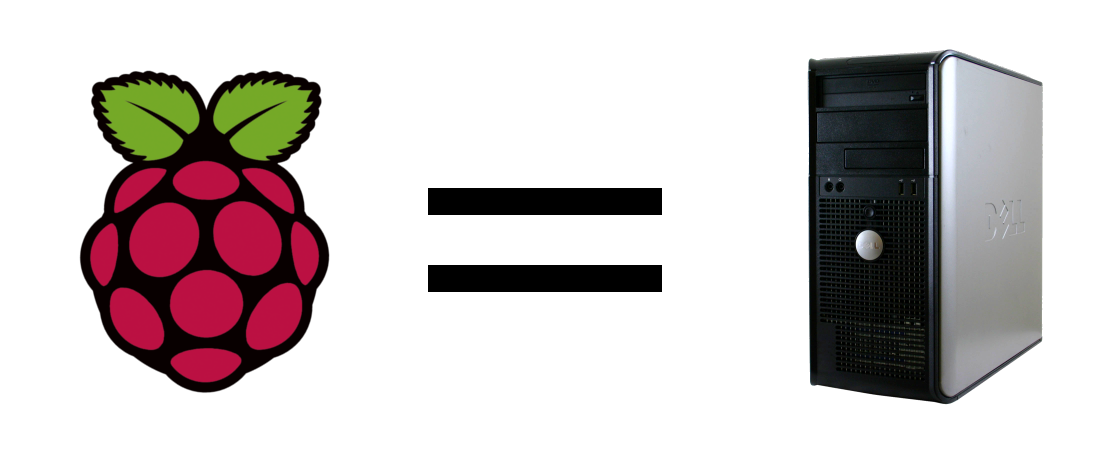
\includegraphics[width=9cm]{isapc.png}
\end{center}
\end{frame}

\begin{frame}{Cosa \`e il Raspberry Pi}

\pause
\begin{block}{}
Il Raspberry Pi \`e a tutti gli effetti un \textbf{computer}, che ci permette sostanzialmente di effettuare le stesse operazioni che faremo con un computer classico.
\end{block}

\pause
\medskip

Ha le stesse prestazioni di un PC di \textbf{inizio anni 2000}, ma:
\pause
\begin{itemize}
\item Consuma di meno.
\pause
\item \`E molto pi\`u piccolo!
\pause
\item Possiamo lasciarlo acceso senza limiti.
\pause
\end{itemize}
\end{frame}

\begin{frame}{Cosa \`e il Raspberry Pi}
\begin{block}{Cosa \`e?}
\emph{
Il Raspberry Pi è un single-board computer (un calcolatore implementato su una sola scheda elettronica).}
\begin{flushright}
\begin{footnotesize}
\emph{Da Wikipedia, l'enciclopedia libera.}
\end{footnotesize}
\end{flushright}

\end{block}

\pause
\medskip

...per\`o \`e pi\`u \textbf{piccolo} e funziona con \textbf{Linux}!

\begin{center}
\visible<2>{
\includegraphics[width=2cm]{tux.png}}
\end{center}

\end{frame}

\begin{frame}{Cosa \`e il Raspberry Pi}
\begin{center}
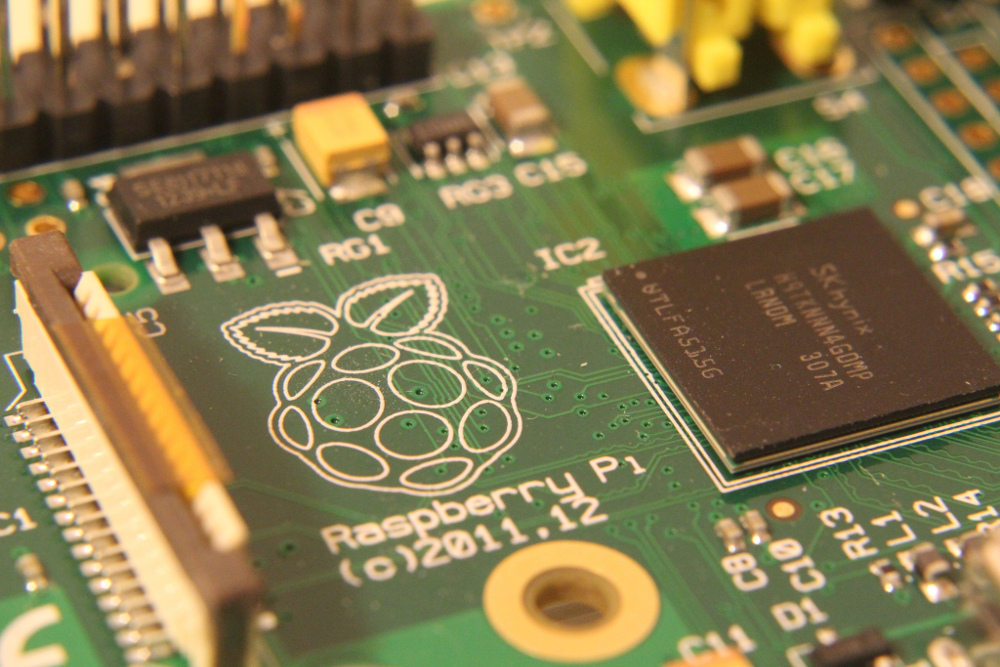
\includegraphics[width=9cm]{raspi-artistic.jpg}
\end{center}
\end{frame}

\subsection{Come nasce?}
\begin{frame}{Come nasce il Raspberry Pi}
\begin{center}

\includegraphics[width=6cm]{logo_raspi.png}
\end{center}
\pause

Il Raspberry Pi nasce nel Regno Unito, realizzato dalla \emph{Raspberry Pi Foundation}

\begin{center}
\url{http://www.raspberrypi.org/}
\end{center}

\pause
\medskip

\begin{block}{}
\`E nato con l'intendo di creare un computer:
\pause
\begin{itemize}
\item Per avvicinare alla programmazione,
\pause
\item Per la didattica nelle scuole,
\pause
\item Che sia economicamente accessibile.
\end{itemize}
\end{block}
\end{frame}

\subsection{Quanto costa?}
\begin{frame}{Quanto costa?}

I vari modelli di Raspberry Pi costanno all'incirca \textbf{35 euro}. Come fa a costare cos\`i poco?

\medskip
\pause

\begin{enumerate}
\item Istruzioni assenti
\pause
\item Case assente
\pause
\item Alimentatore assente
\pause
\item SD assente
\pause
\item Pulsante di accensione assente
\end{enumerate}

\visible<7>{
\begin{center}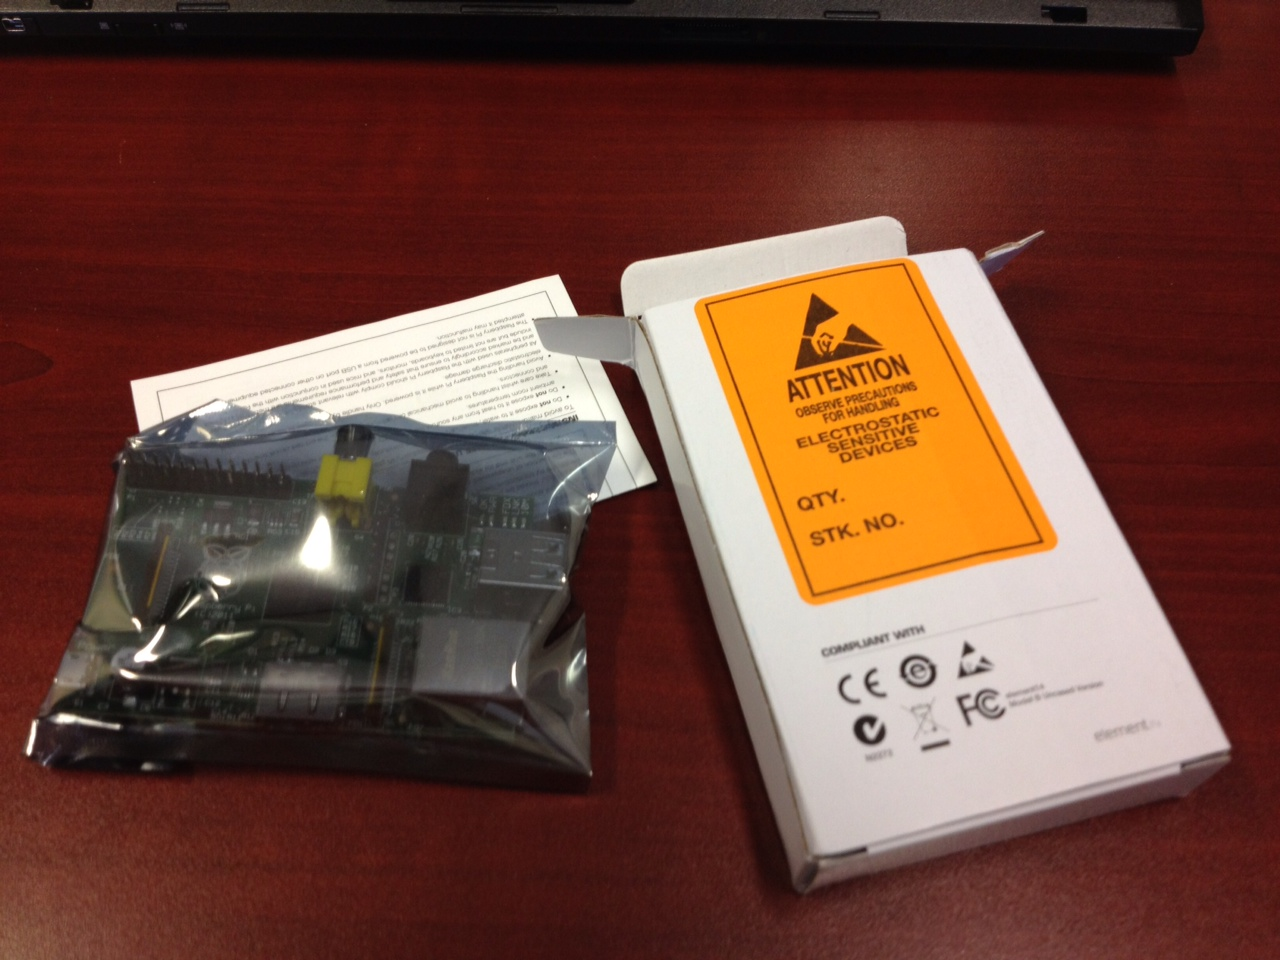
\includegraphics[width=4cm]{box.png}\end{center}
}

\end{frame}


\section{Modelli di Raspberry}

\begin{frame}{Raspberry Pi - Model A}
\begin{center}
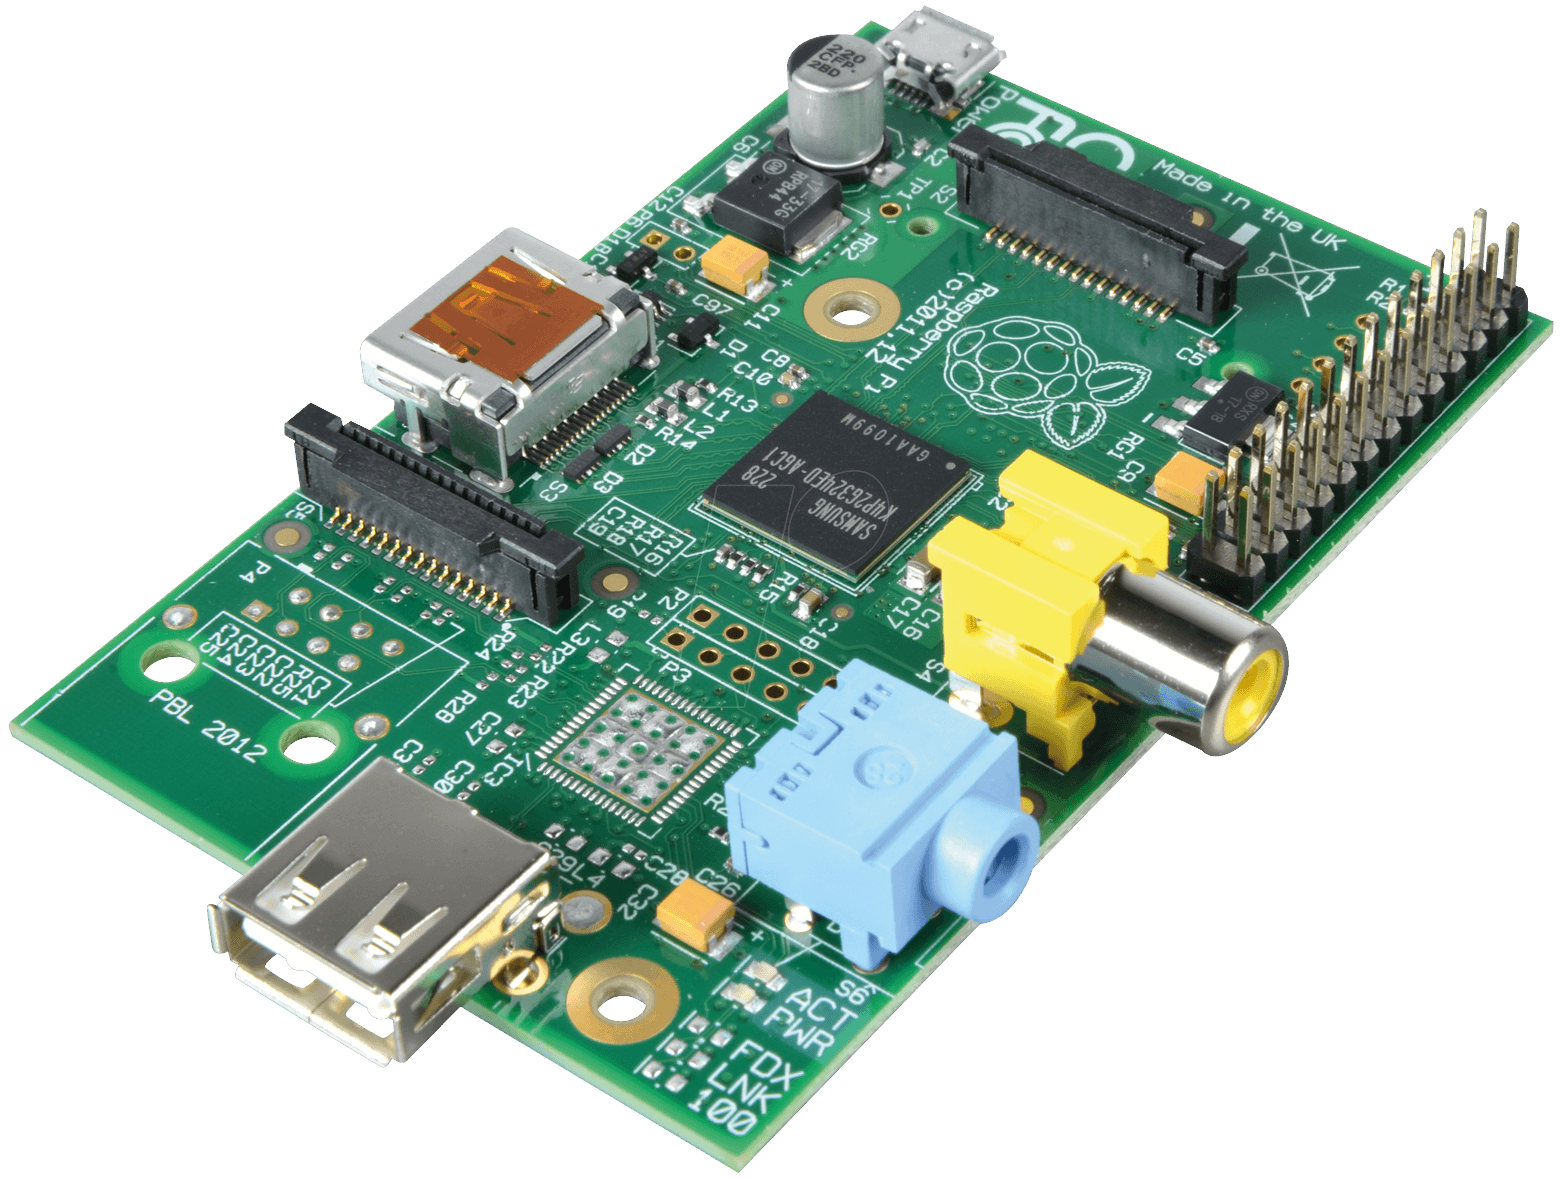
\includegraphics[width=9cm]{raspiA.png}
\end{center}
\end{frame}

\begin{frame}{Raspberry Pi - Model A+}
\begin{center}
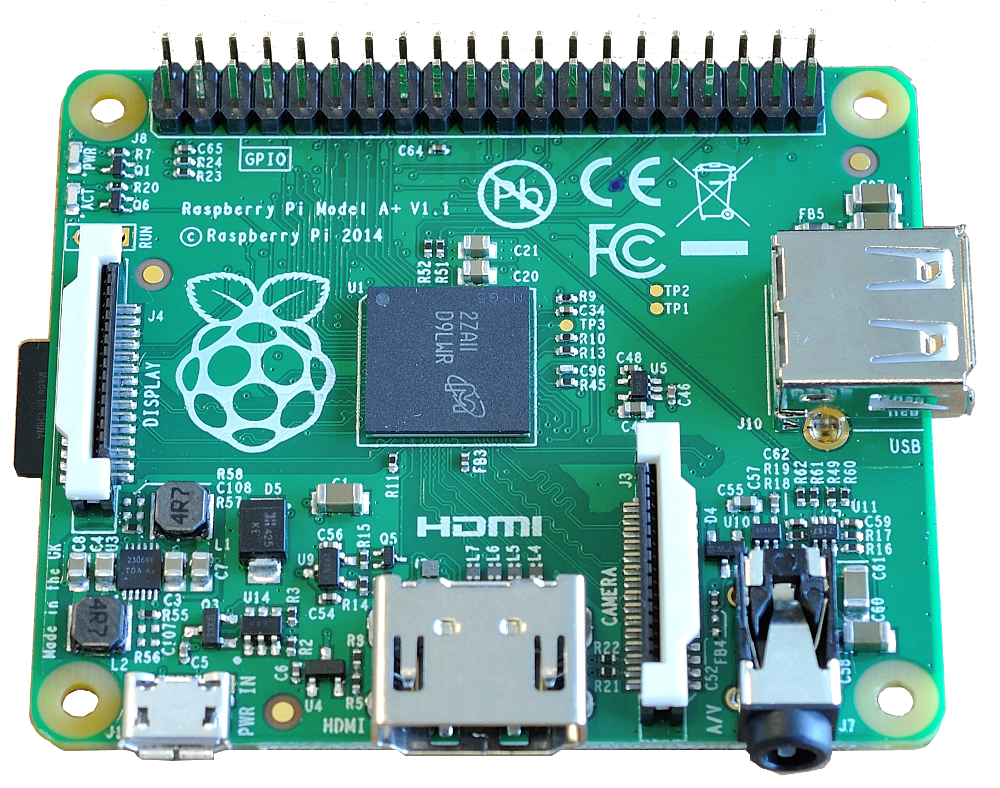
\includegraphics[width=9cm]{raspiA+.png}
\end{center}
\end{frame}

\begin{frame}{Raspberry Pi - Model B}
\begin{center}
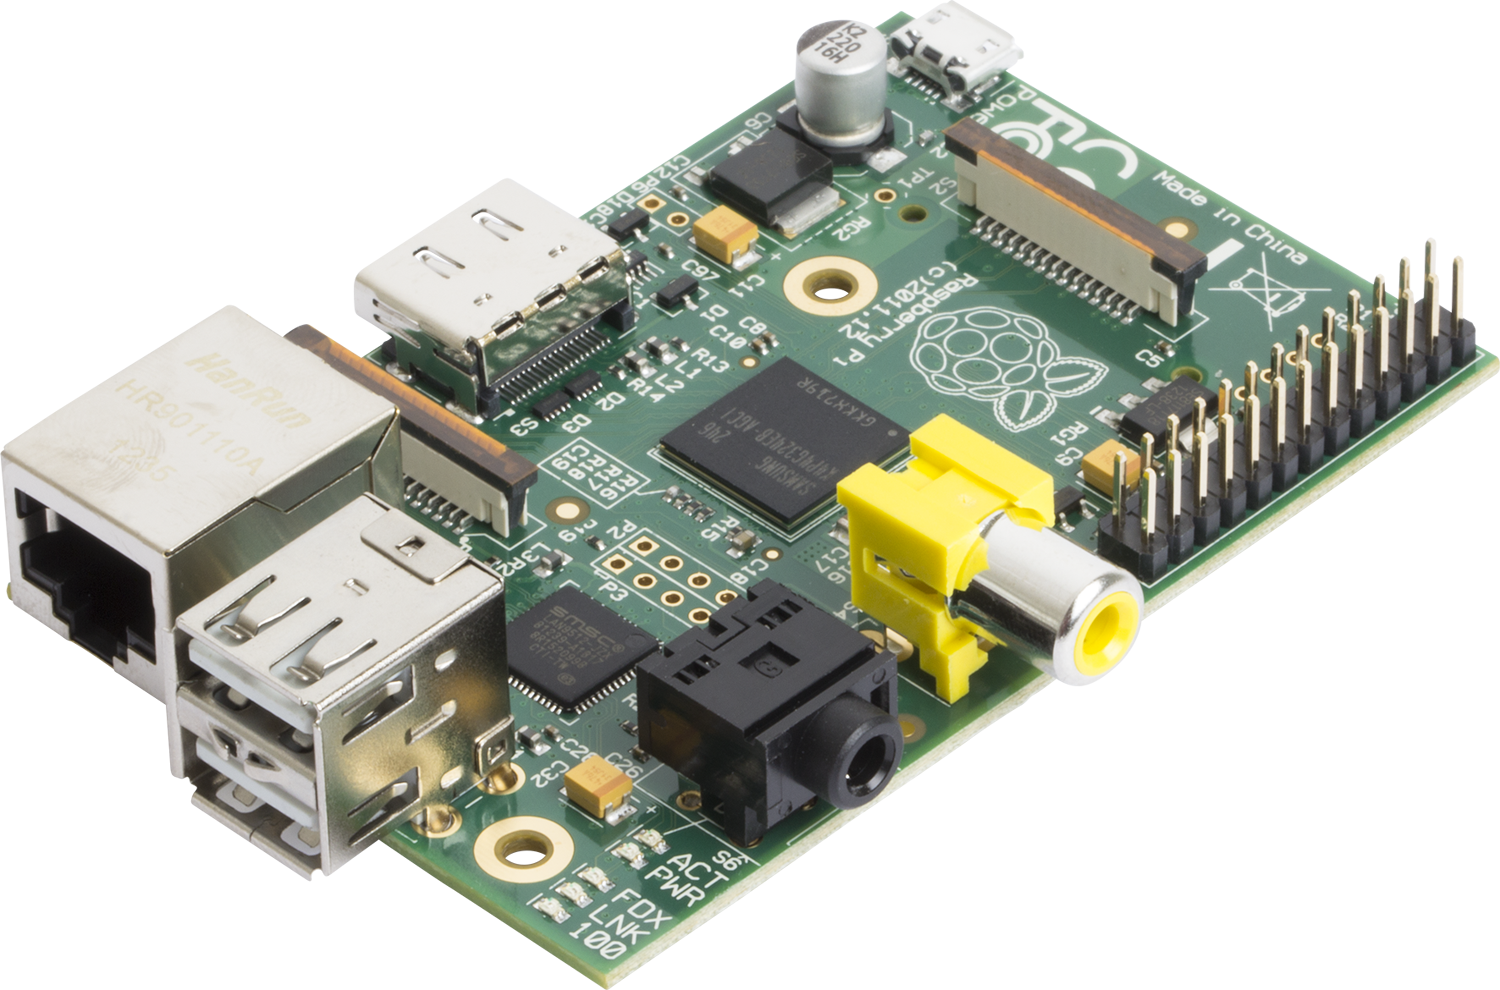
\includegraphics[width=9cm]{raspiB.png}
\end{center}
\end{frame}

\begin{frame}{Raspberry Pi - Model B+}
\begin{center}
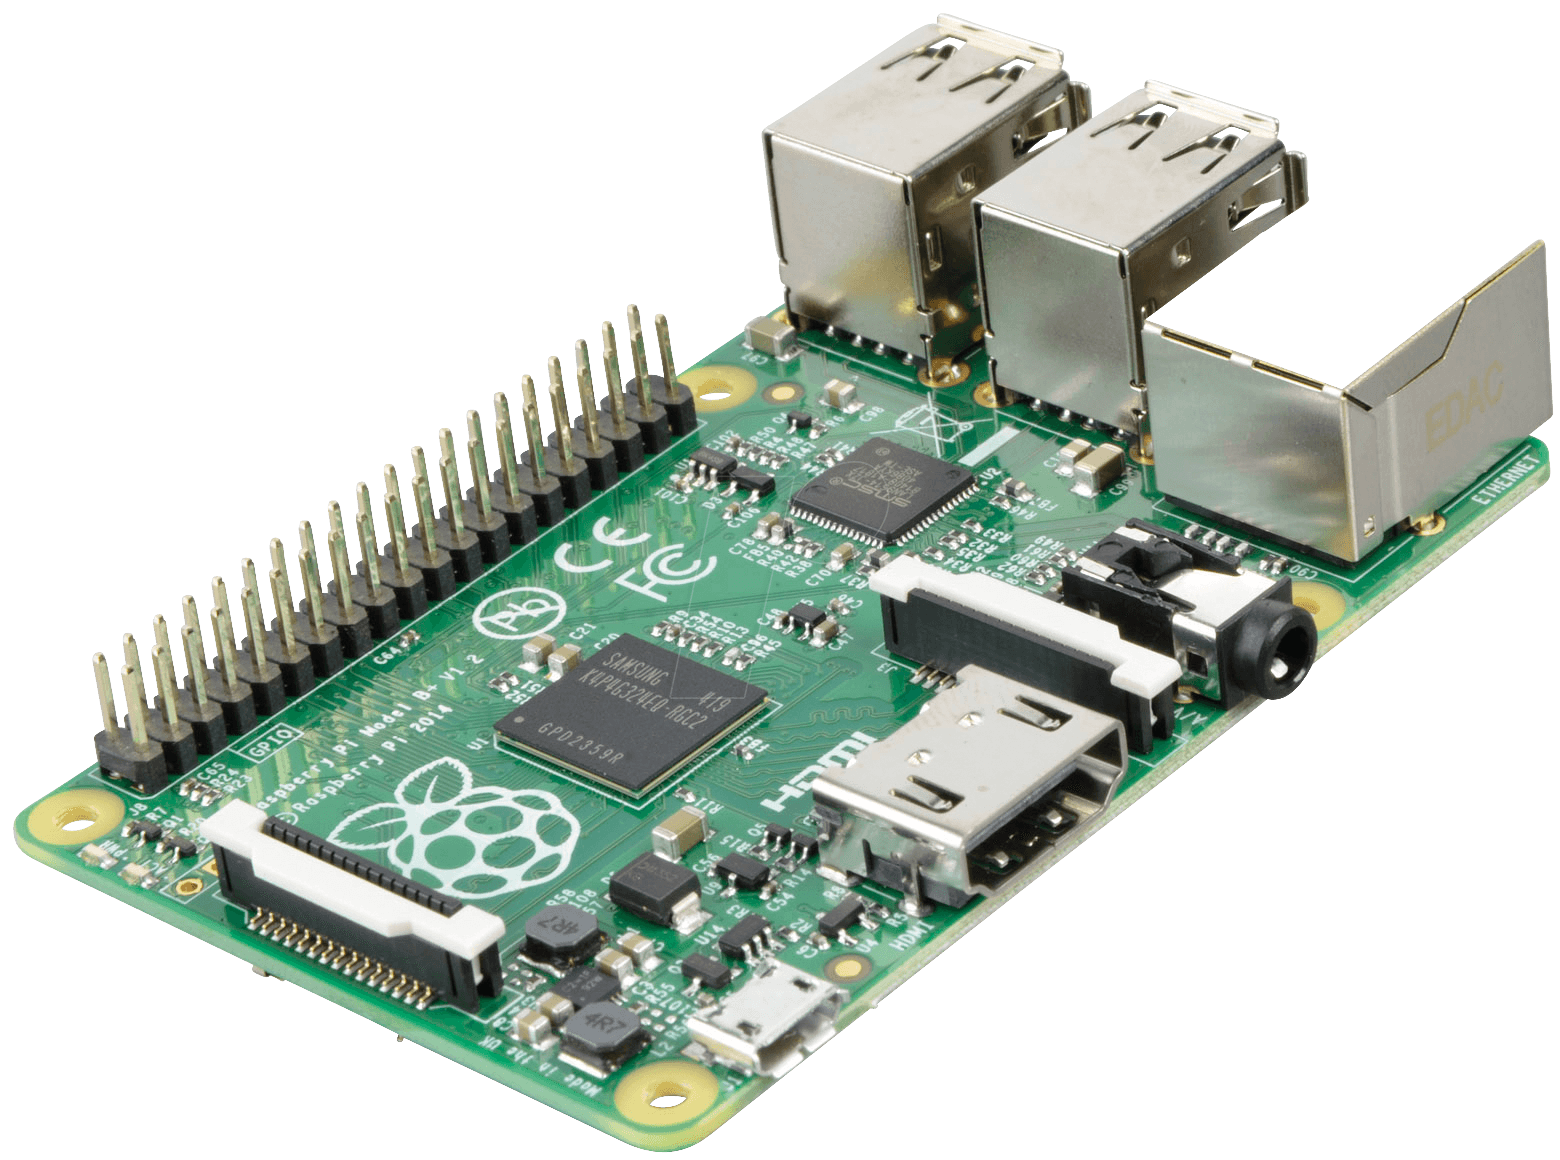
\includegraphics[width=9cm]{raspiB+.png}
\end{center}
\end{frame}

\begin{frame}{Raspberry Pi 2 - Model B}
\begin{center}
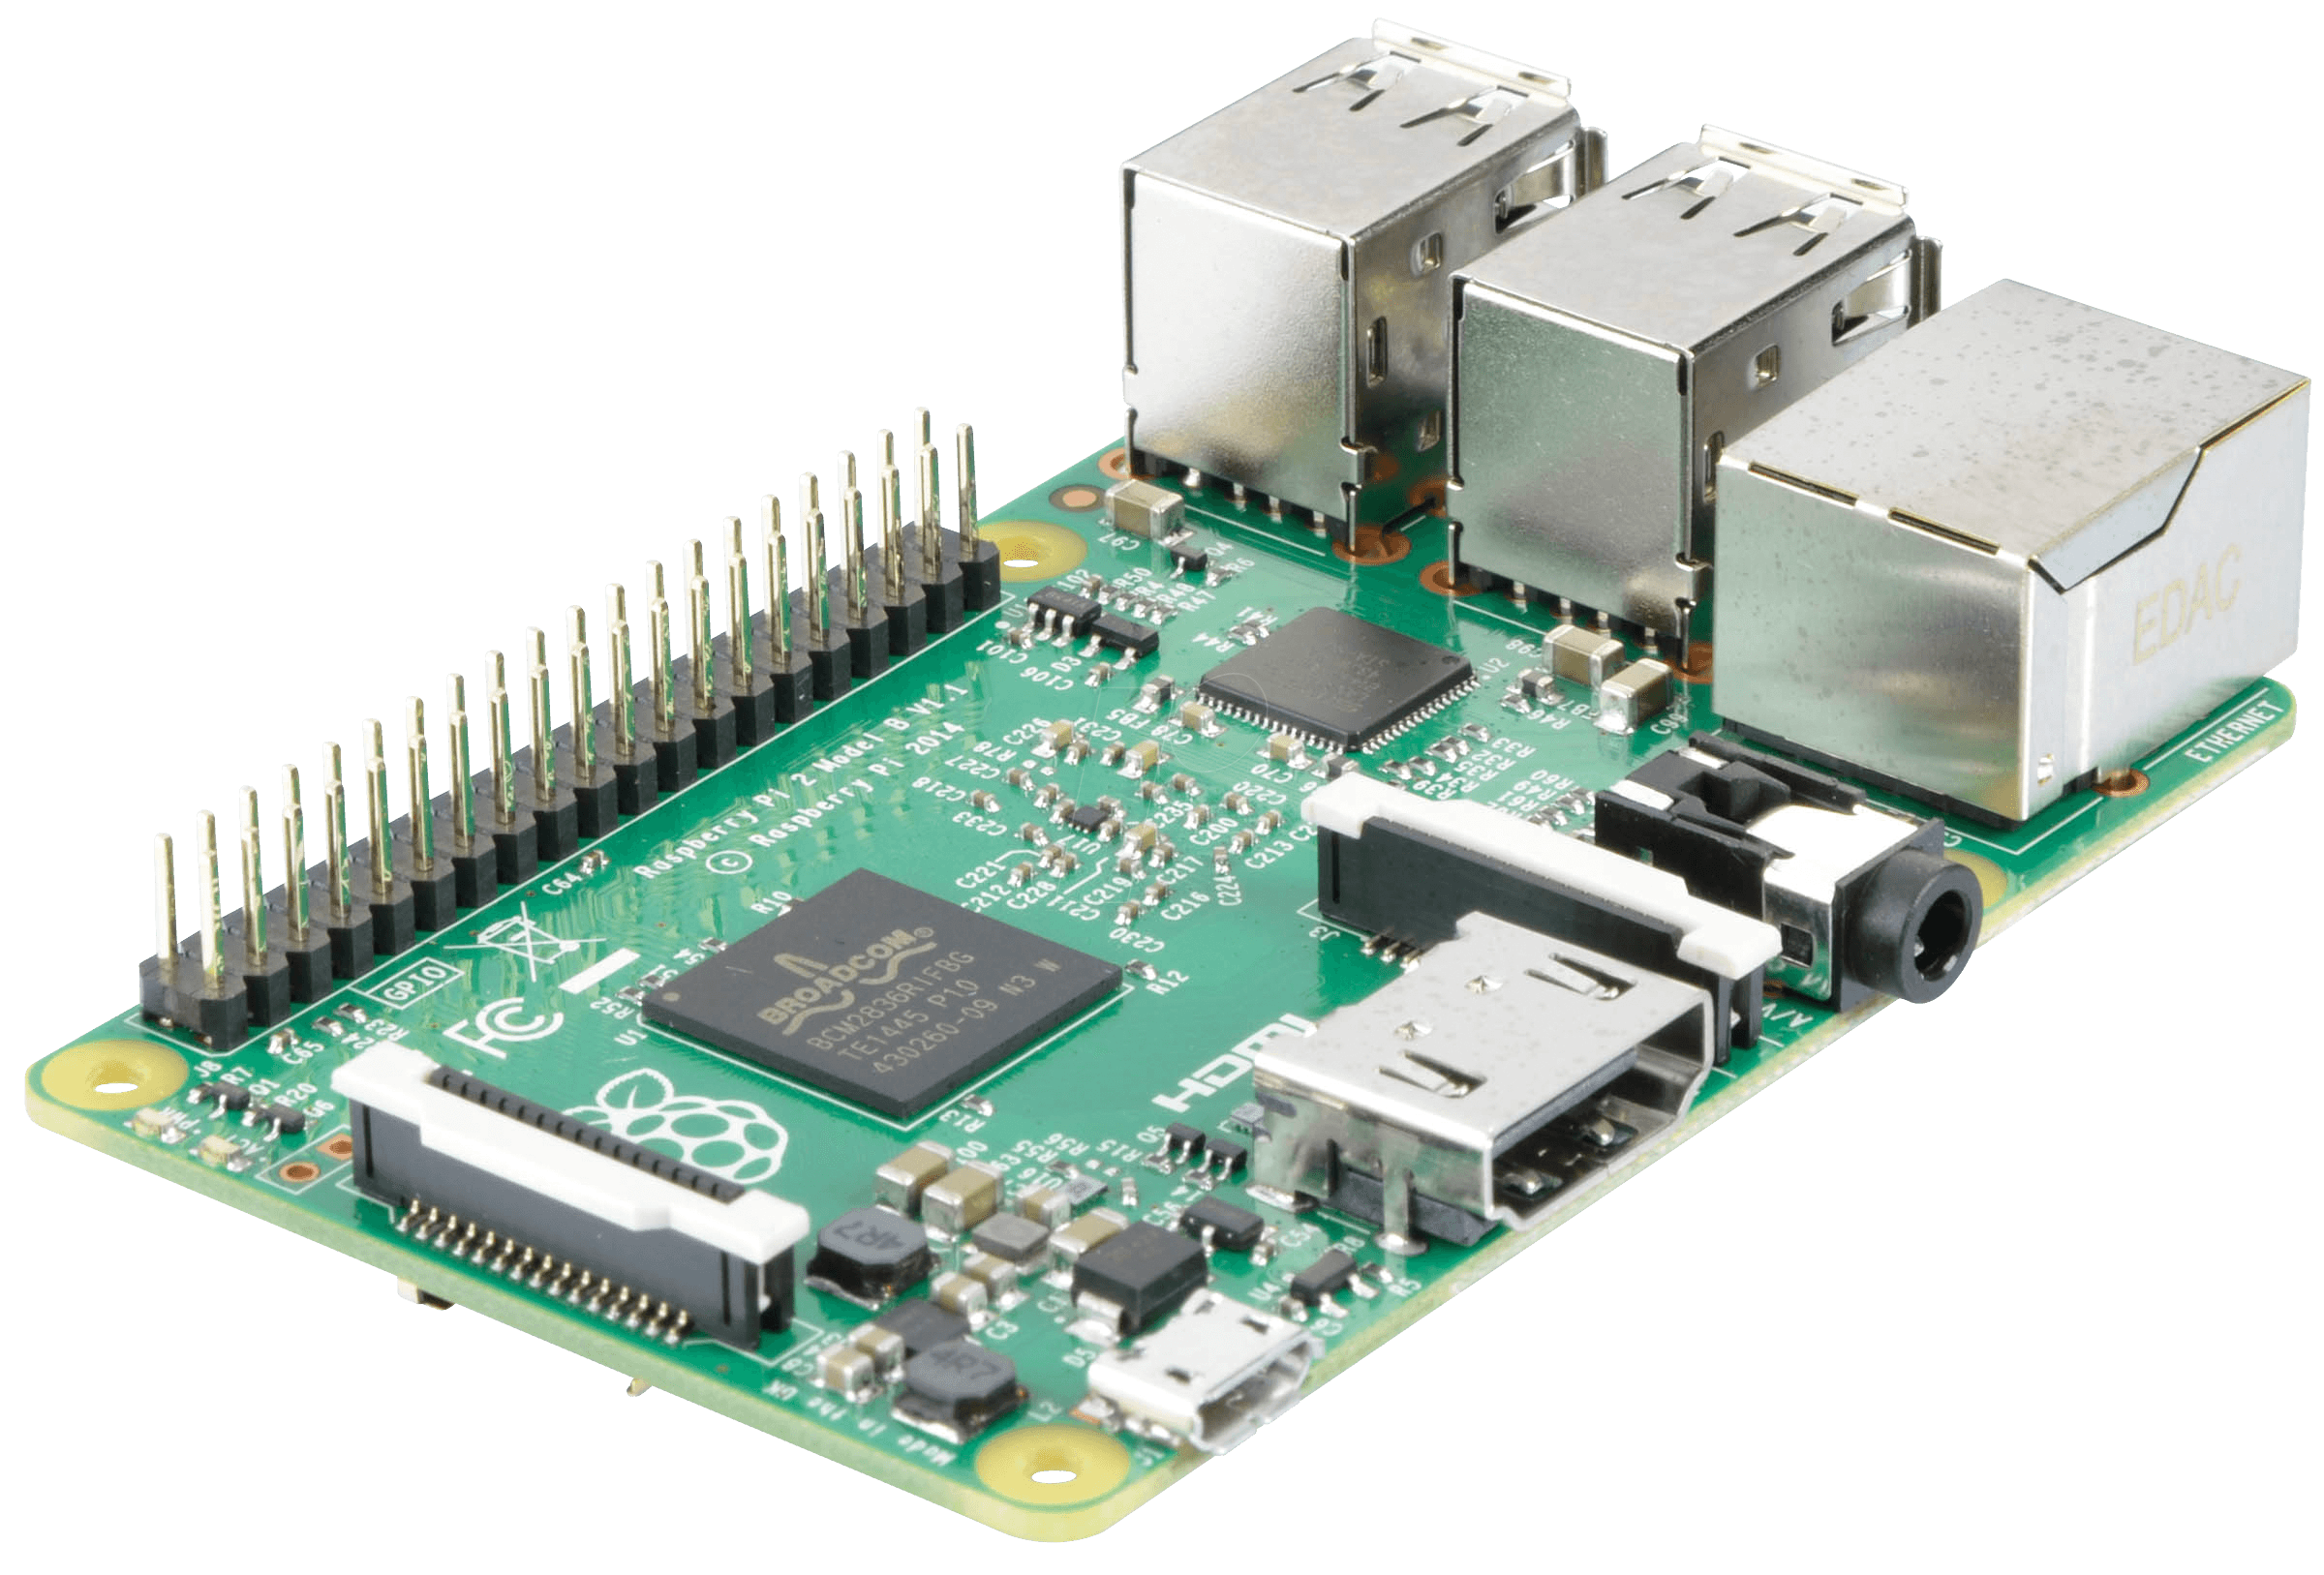
\includegraphics[width=9cm]{raspi2.png}
\end{center}
\end{frame}

\subsection{Tech specs}
\begin{frame}[fragile]{Specifiche tecniche}
\begin{center}
\begin{tabular}{|c|c|c|c|c|c|}
\hline
 & \textbf{A} & \textbf{A+} & \textbf{B} & \textbf{B+} & \textbf{2} \\
\hline
\textbf{CPU} & \multicolumn{4}{c|}{{\tiny BMC2835 700 MHz ARM11}} & {\tiny BCM2836 900 MHz A7} \\
\hline
\textbf{GPU} & \multicolumn{5}{c|}{{\tiny Broadcom VideoCore IV, OpenGL ES 2.0, 1080p H.264 decode}} \\
\hline
\textbf{RAM} & \multicolumn{2}{c|}{{\tiny 256 Mb shared}} & \multicolumn{2}{c|}{{\tiny 512 Mb shared}} & {\tiny 1 Gb shared}\\
\hline
\textbf{USB} & \multicolumn{2}{c|}{{\tiny 1}} & {\tiny 2 (HUB)} & \multicolumn{2}{c|}{{\tiny 4 (HUB)}} \\
\hline
\textbf{SD} & {\tiny SD/MMC} & {\tiny micro SD} & {\tiny SD/MMC} & \multicolumn{2}{c|}{{\tiny micro SD}} \\
\hline
\textbf{Video} & \multicolumn{5}{c|}{{\tiny RCA and HDMI ports}} \\
\hline
\textbf{Audio} & \multicolumn{5}{c|}{{\tiny 3,5 mm jack and HDMI}} \\
\hline
\textbf{Network} & \multicolumn{2}{c|}{{\tiny None}} & \multicolumn{3}{c|}{{\tiny Ethernet 10/100 (RJ45)}}\\
\hline
\end{tabular}
\end{center}
\end{frame}

\begin{frame}[fragile]{Specifiche tecniche}
\begin{center}
\begin{tabular}{|c|c|c|c|c|c|}
\hline
 & \textbf{A} & \textbf{A+} & \textbf{B} & \textbf{B+} & \textbf{2} \\
\hline
\textbf{Video in} & \multicolumn{5}{c|}{{\tiny 15-pin MIPI camera interface (CSI) connector}} \\
\hline
\textbf{Audio in} & \multicolumn{5}{c|}{{\tiny From revision 2 boards through I²S}} \\
\hline
\textbf{Clock} & \multicolumn{5}{c|}{{\tiny No clock or battery}} \\
\hline 
\textbf{GPIO} & {\tiny 26 pins} & {\tiny 40 pins} & {\tiny 26 pins} & \multicolumn{2}{c|}{{\tiny 40 pins}} \\
\hline
\textbf{Power} & {\tiny 300 mA} & {\tiny 200 mA} & {\tiny 700 mA} & {\tiny 600 mA} & {\tiny 800 mA} \\
\hline
\textbf{Weight} & {\tiny 45 g} & {\tiny 23 g} & \multicolumn{3}{c|}{{\tiny 45 g}} \\
\hline
\textbf{Size} & {\tiny 85 × 56 mm } & {\tiny 65 × 56 mm } & \multicolumn{3}{c|}{{\tiny 85 × 56 mm}} \\
\hline
\textbf{Price} & {\tiny 25 \$} & {\tiny 20 \$} & \multicolumn{3}{c|}{{\tiny 35 \$}} \\
\hline
\end{tabular}
\end{center}
\end{frame}

\begin{frame}{GPIO}
\begin{center}
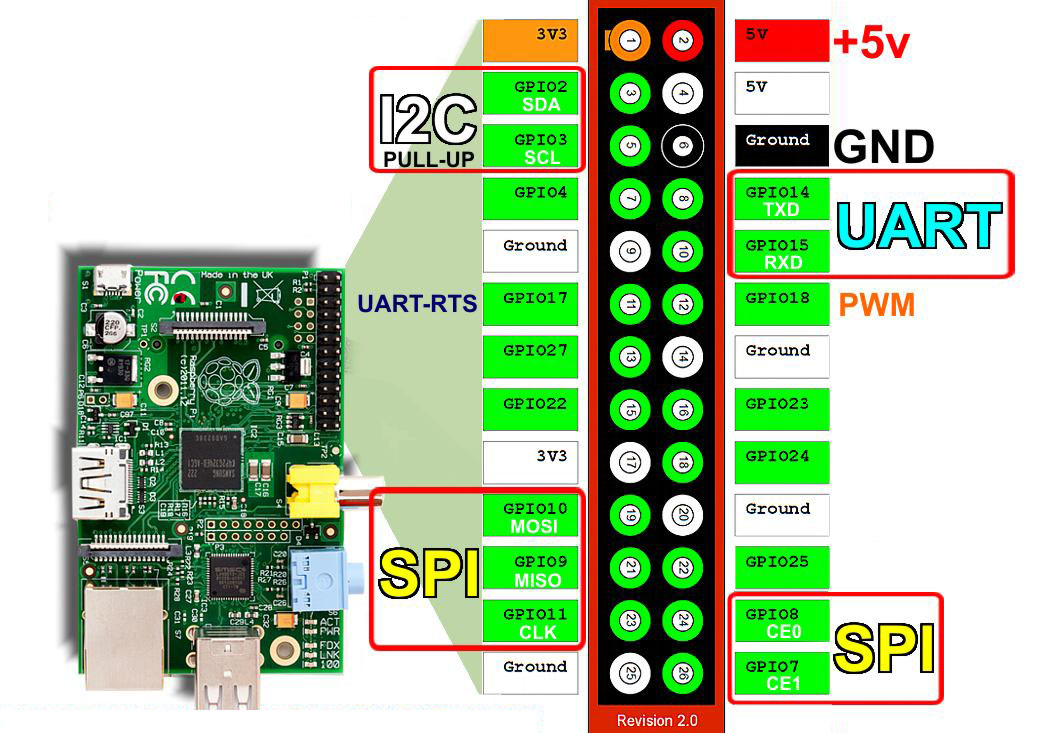
\includegraphics[width=9cm]{gpio.jpg}
\end{center}
\end{frame}

\section{Accessori}

\subsection{Essenziali}
\begin{frame}{La lista della spesa}
Per iniziare a divertirci con il nostro Raspberry Pi avremo bisogno di:
\pause
\begin{description}
\item[{\color{green_raspi} Alimentatore}] Micro USB, Output a 1200 $mA$.
\pause
\item[{\color{green_raspi} Scheda SD}] Da almeno 4 GB, meglio se da 8 GB (e possibilmente di classe 10).
\pause
\item[{\color{green_raspi} Rete}] Connessione ethernet ad internet.
\pause
\item[{\color{green_raspi} Input}] Mouse e tastiera USB (consigliati).
\pause
\item[{\color{green_raspi} Monitor}] Con interfaccia HDMI o DVI (consigliati), oppure un televisore con entrata RCA.
\end{description}
\end{frame}

\begin{frame}{Pi Starter Kit}
\begin{center}
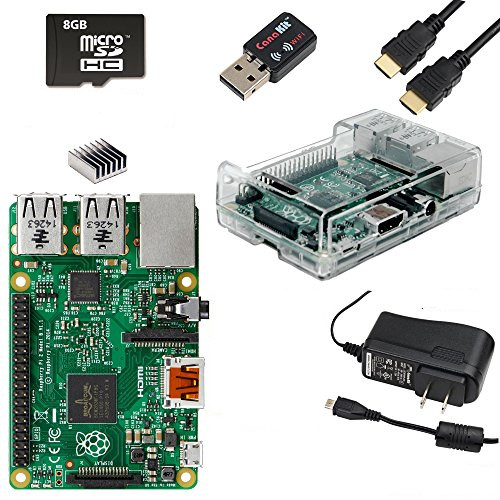
\includegraphics[width=8cm]{kit.jpg}
\end{center}
\end{frame}

\subsection{Addons}
\begin{frame}[fragile]{Accessori per il Raspberry Pi}
Estendiamo il nostro Raspberry Pi tramite:
\vspace{1cm}

\begin{columns}
    \begin{column}{0.5\textwidth}
	\begin{itemize}
	\item Pi-Camera
	\pause
	\item Touch Screen LCD
	\pause
	\item Hub USB
	\pause
	\item Dongle Wifi (Bluetooth o 3G)
	\pause
	\item Case
	\end{itemize}
    \end{column}
    \begin{column}{0.5\textwidth}
    \begin{center}
      \includegraphics<1>[height=4cm]{picamera.png}
      \includegraphics<2>[height=4cm]{pimonitor.png}
      \includegraphics<3>[height=4cm]{pihub.png}
      \includegraphics<4>[height=4cm]{piwifi.png}
      \includegraphics<5>[height=4cm]{picase.png}            
    \end{center}
    \end{column}
  \end{columns}
\end{frame}

\section{Dove Comprare}

\begin{frame}{Dove comprare il Raspberry Pi}

\begin{center}

\includegraphics[width=5cm]{wherebuy.png}
\end{center}

\`E possibile acquistare il Raspberry Pi presso uno dei distributori ufficiali, oppure anche su qualsiasi altro shop online che venda articoli di elettronica.
\end{frame}

\section{Distribuzioni Linux}

\begin{frame}{}
\begin{center}
\begin{Huge}
{\color{green_raspi} \textbf{Distribuzioni Linux}}
\end{Huge}
\end{center}
\end{frame}

\begin{frame}{Raspbian}
\begin{center}

\includegraphics[width=6cm]{raspbian_logo.png}
\end{center}

\pause
\medskip

\begin{block}{Raspbian}
\textbf{Raspbian} \`e una versione modificata di \emph{Debian Wheezy} (una delle pi\`u famose distribuzioni di Linux) ottimizzata per architettura \textbf{arm}. L'ambiente desktop di default \`e \textbf{LXDE}
\end{block}

\pause
\medskip

Raspbian fornisce un insieme molto grande di pacchetti gi\`a funzionanti per Raspberry Pi, installabili tramite il famoso comando \texttt{apt-get install}.

\pause
\medskip
\begin{center}
\url{http://www.raspbian.org/}
\end{center}
\end{frame}

\begin{frame}{Raspbian}
\begin{center}
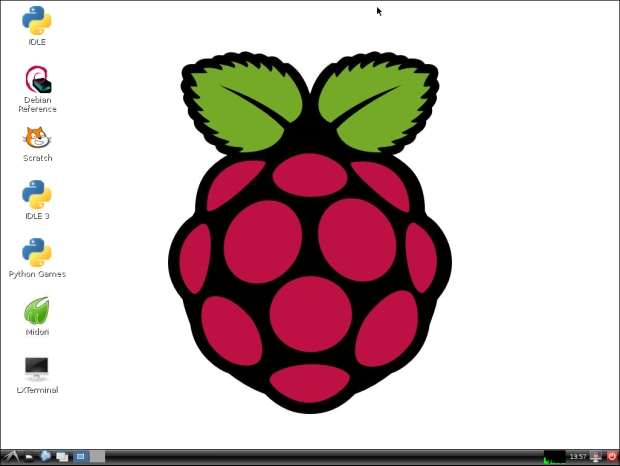
\includegraphics[width=9cm]{raspbian-desktop.jpg}
\end{center}
\end{frame}


\begin{frame}{Raspbian}

Raspbian mette a disposizione il comando \texttt{raspi-config} per configurare tutti gli aspetti del proprio Raspberry Pi.

\begin{center}
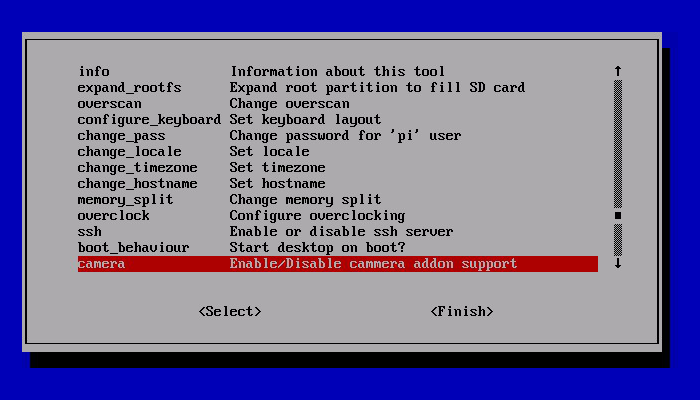
\includegraphics[width=8cm]{raspi-config.png}
\end{center}

\end{frame}

\begin{frame}{Pidora}
\begin{center}

\includegraphics[width=6cm]{pidora.png}
\end{center}

\medskip
\pause

Versione ``alleggerita'' di \textbf{Fedora}, compilata per girare su piattaforma ARM.

\medskip
\pause

\textbf{XFCE} Ambiente desktop di default. \textbf{RPM} Package Manager.

\pause
\medskip
\begin{center}
\url{http://www.pidora.ca/}
\end{center}
\end{frame}

\begin{frame}{Pidora}
\begin{center}
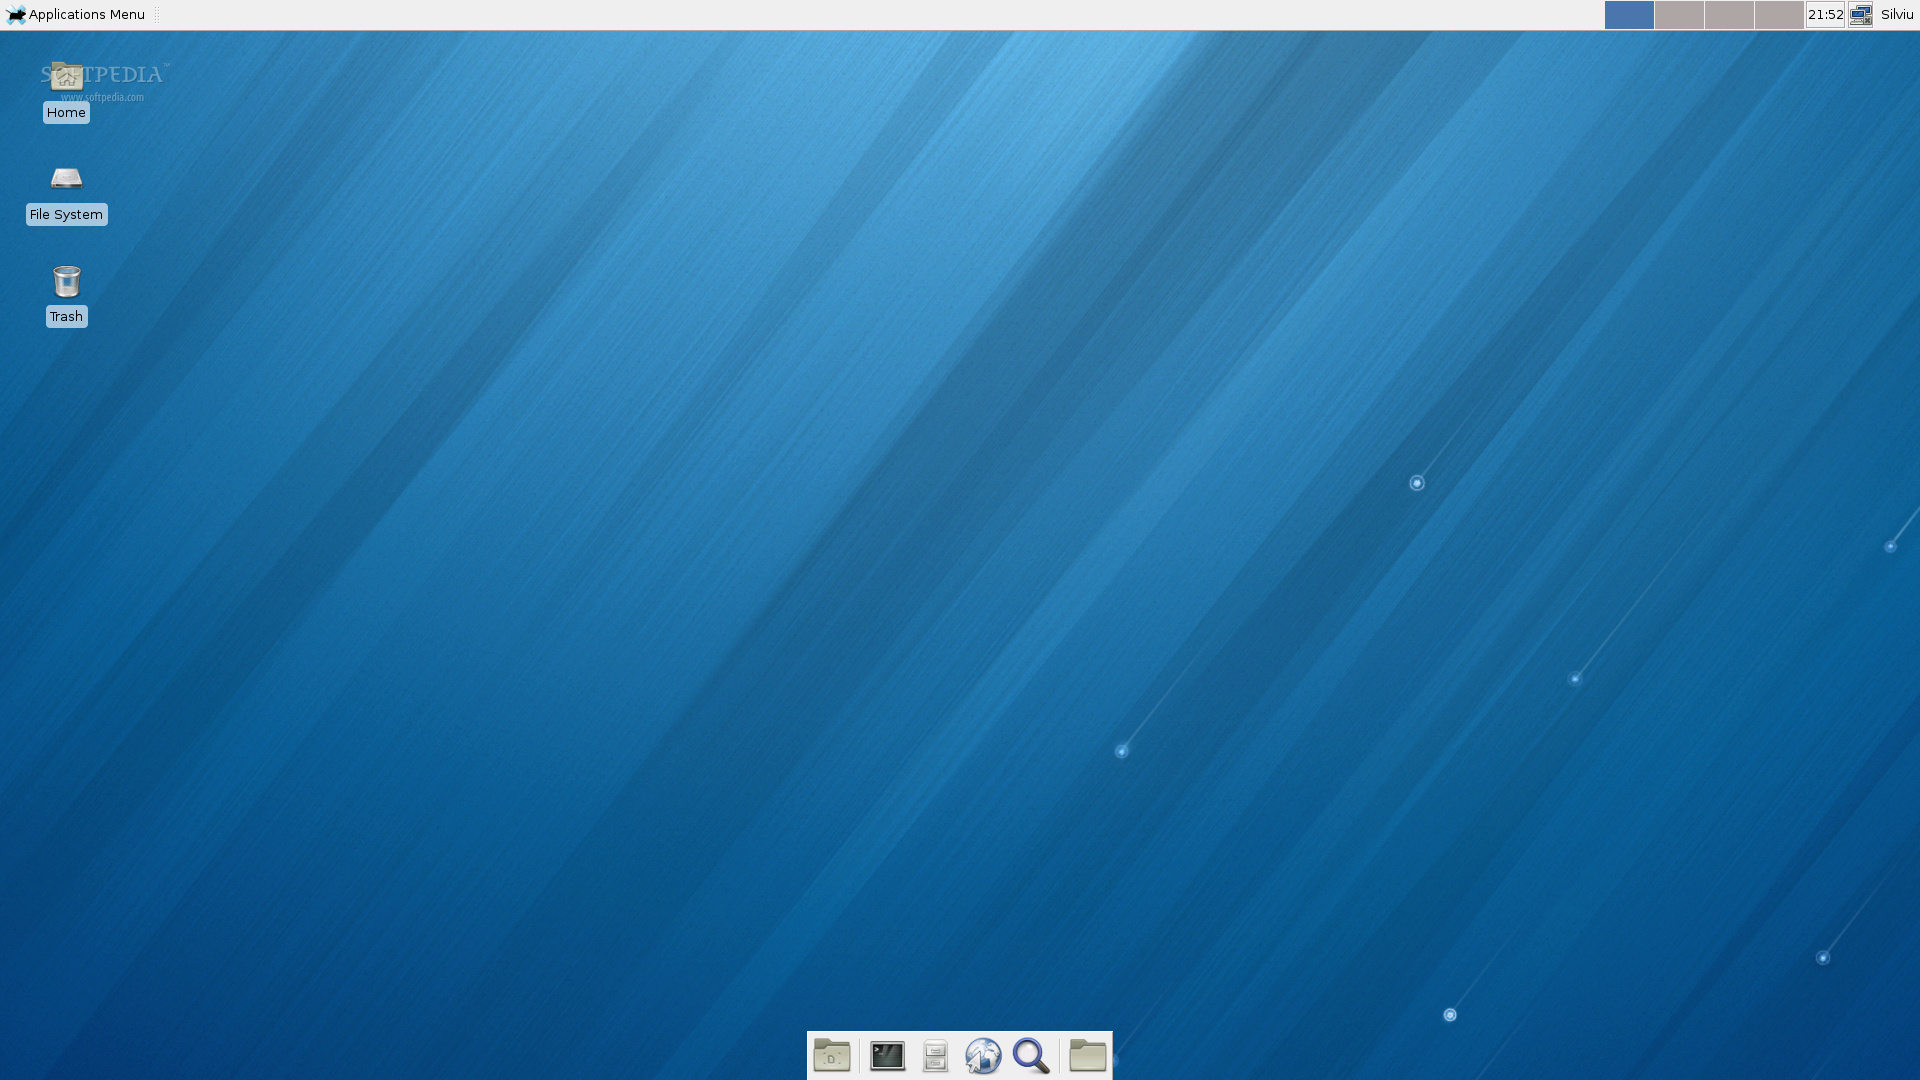
\includegraphics[width=9cm]{pidora-desktop.jpg}
\end{center}
\end{frame}

\begin{frame}[fragile]{Raspbmc - OpenELEC}

\begin{columns}
    \begin{column}{0.5\textwidth}
    \begin{center}
    
    
\includegraphics[height=2cm]{raspbmc_logo.png}

    \end{center}	
	\end{column}

    \begin{column}{0.5\textwidth}
    \begin{center}
    
    
\includegraphics[height=2cm]{open_elec.png}

    \end{center}	
	\end{column}
\end{columns}

\bigskip
\pause

\textbf{Raspbmc} ed \textbf{OpenELEC} sono due distribuzioni che 	forniscono il media center \textbf{XBMC}, che permette di trasformare il vostro Raspberry Pi in un media center domestico.

\pause
\medskip

Il chip grafico del Raspberry Pi permette di fare il decoding di filmati in formato \textbf{H.264} fino a \textbf{1080p}.

\pause
\begin{center}
\url{http://www.raspbmc.com/} \\
\url{http://openelec.tv/}
\end{center}

\end{frame}

\section{Use cases}

\begin{frame}{}
\begin{center}
\begin{Huge}
{\color{green_raspi} \textbf{Use Cases}}
\end{Huge}
\end{center}

\end{frame}

\begin{frame}{Media Center}
\begin{center}
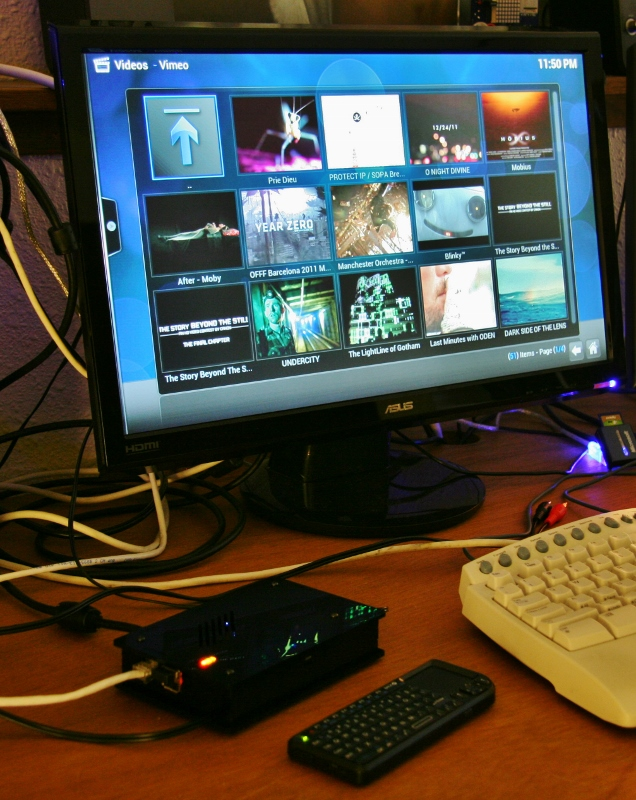
\includegraphics[height=7cm]{uc/media.jpg}
\end{center}
\end{frame}

\begin{frame}{Computer Domestico}
\begin{center}
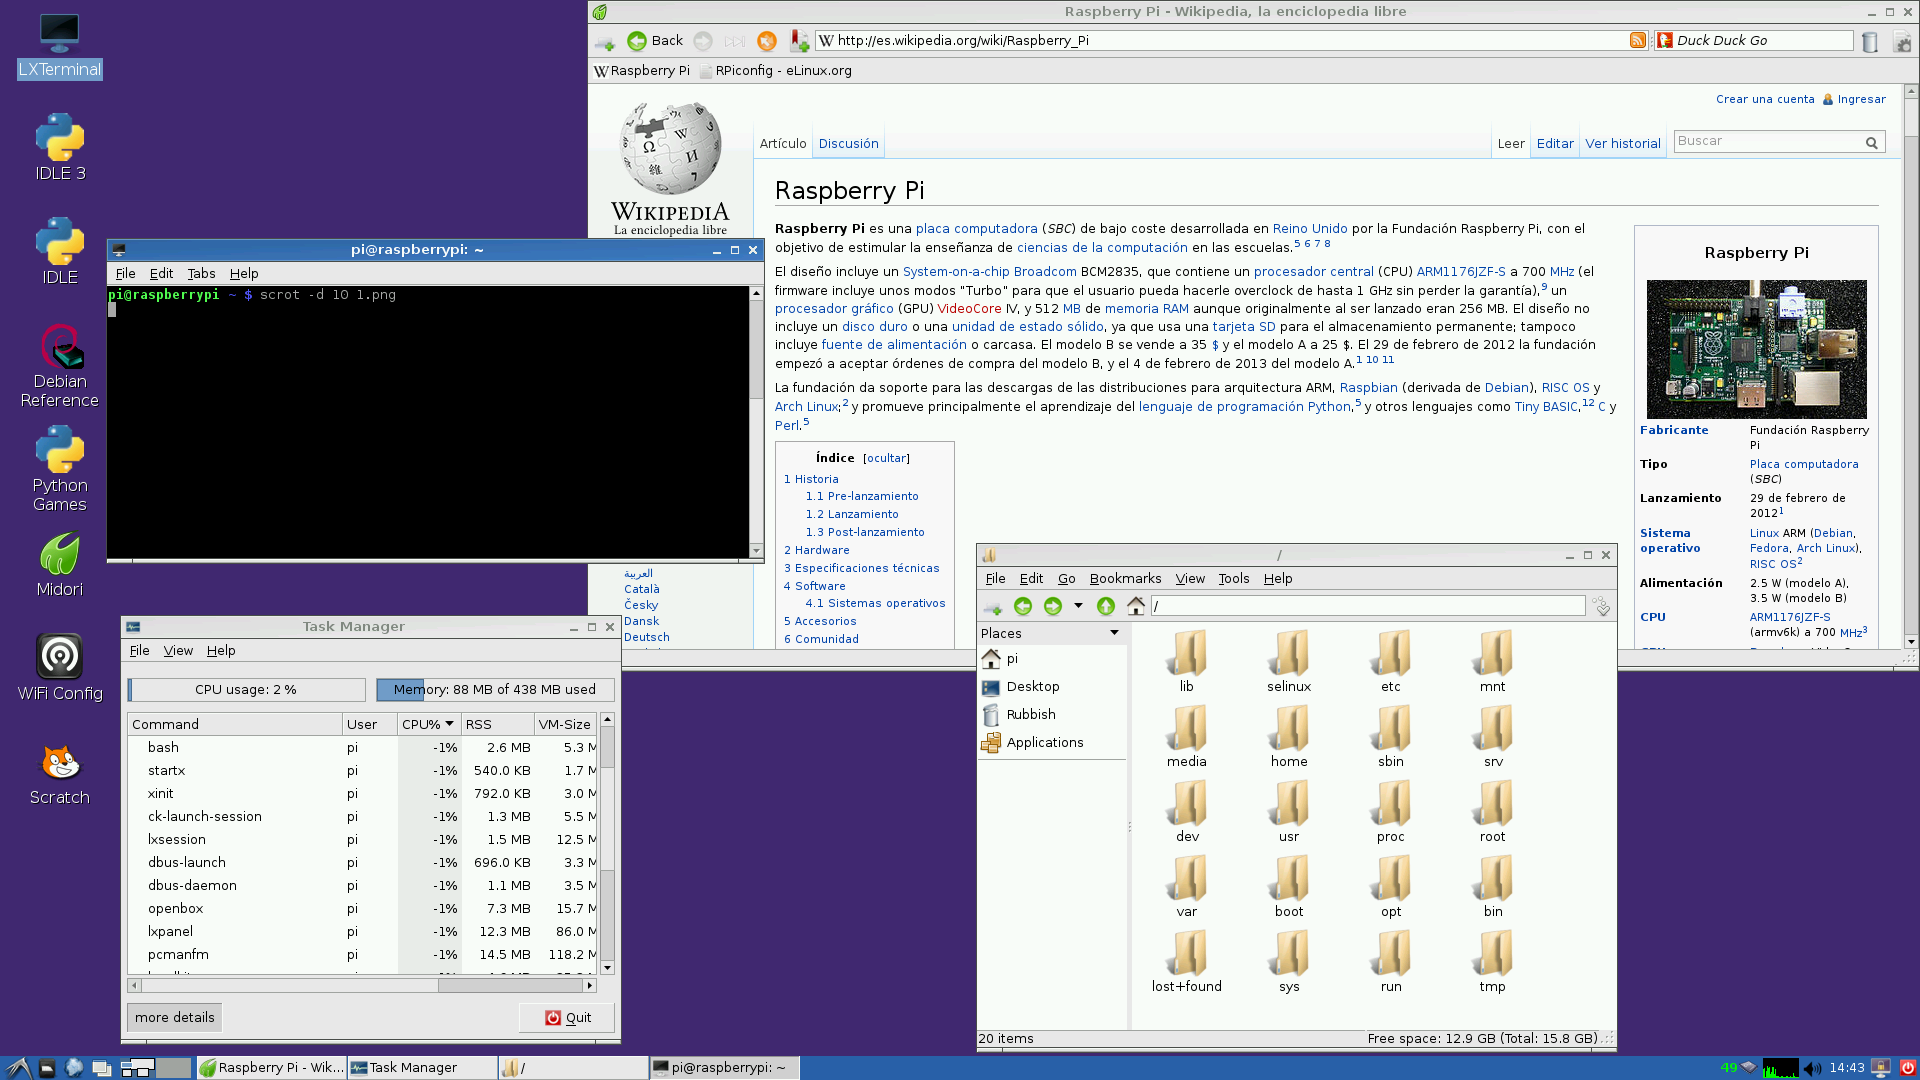
\includegraphics[width=9cm]{uc/pc.png}
\end{center}
\end{frame}

\begin{frame}{Message Board/Kiosk}
\begin{center}
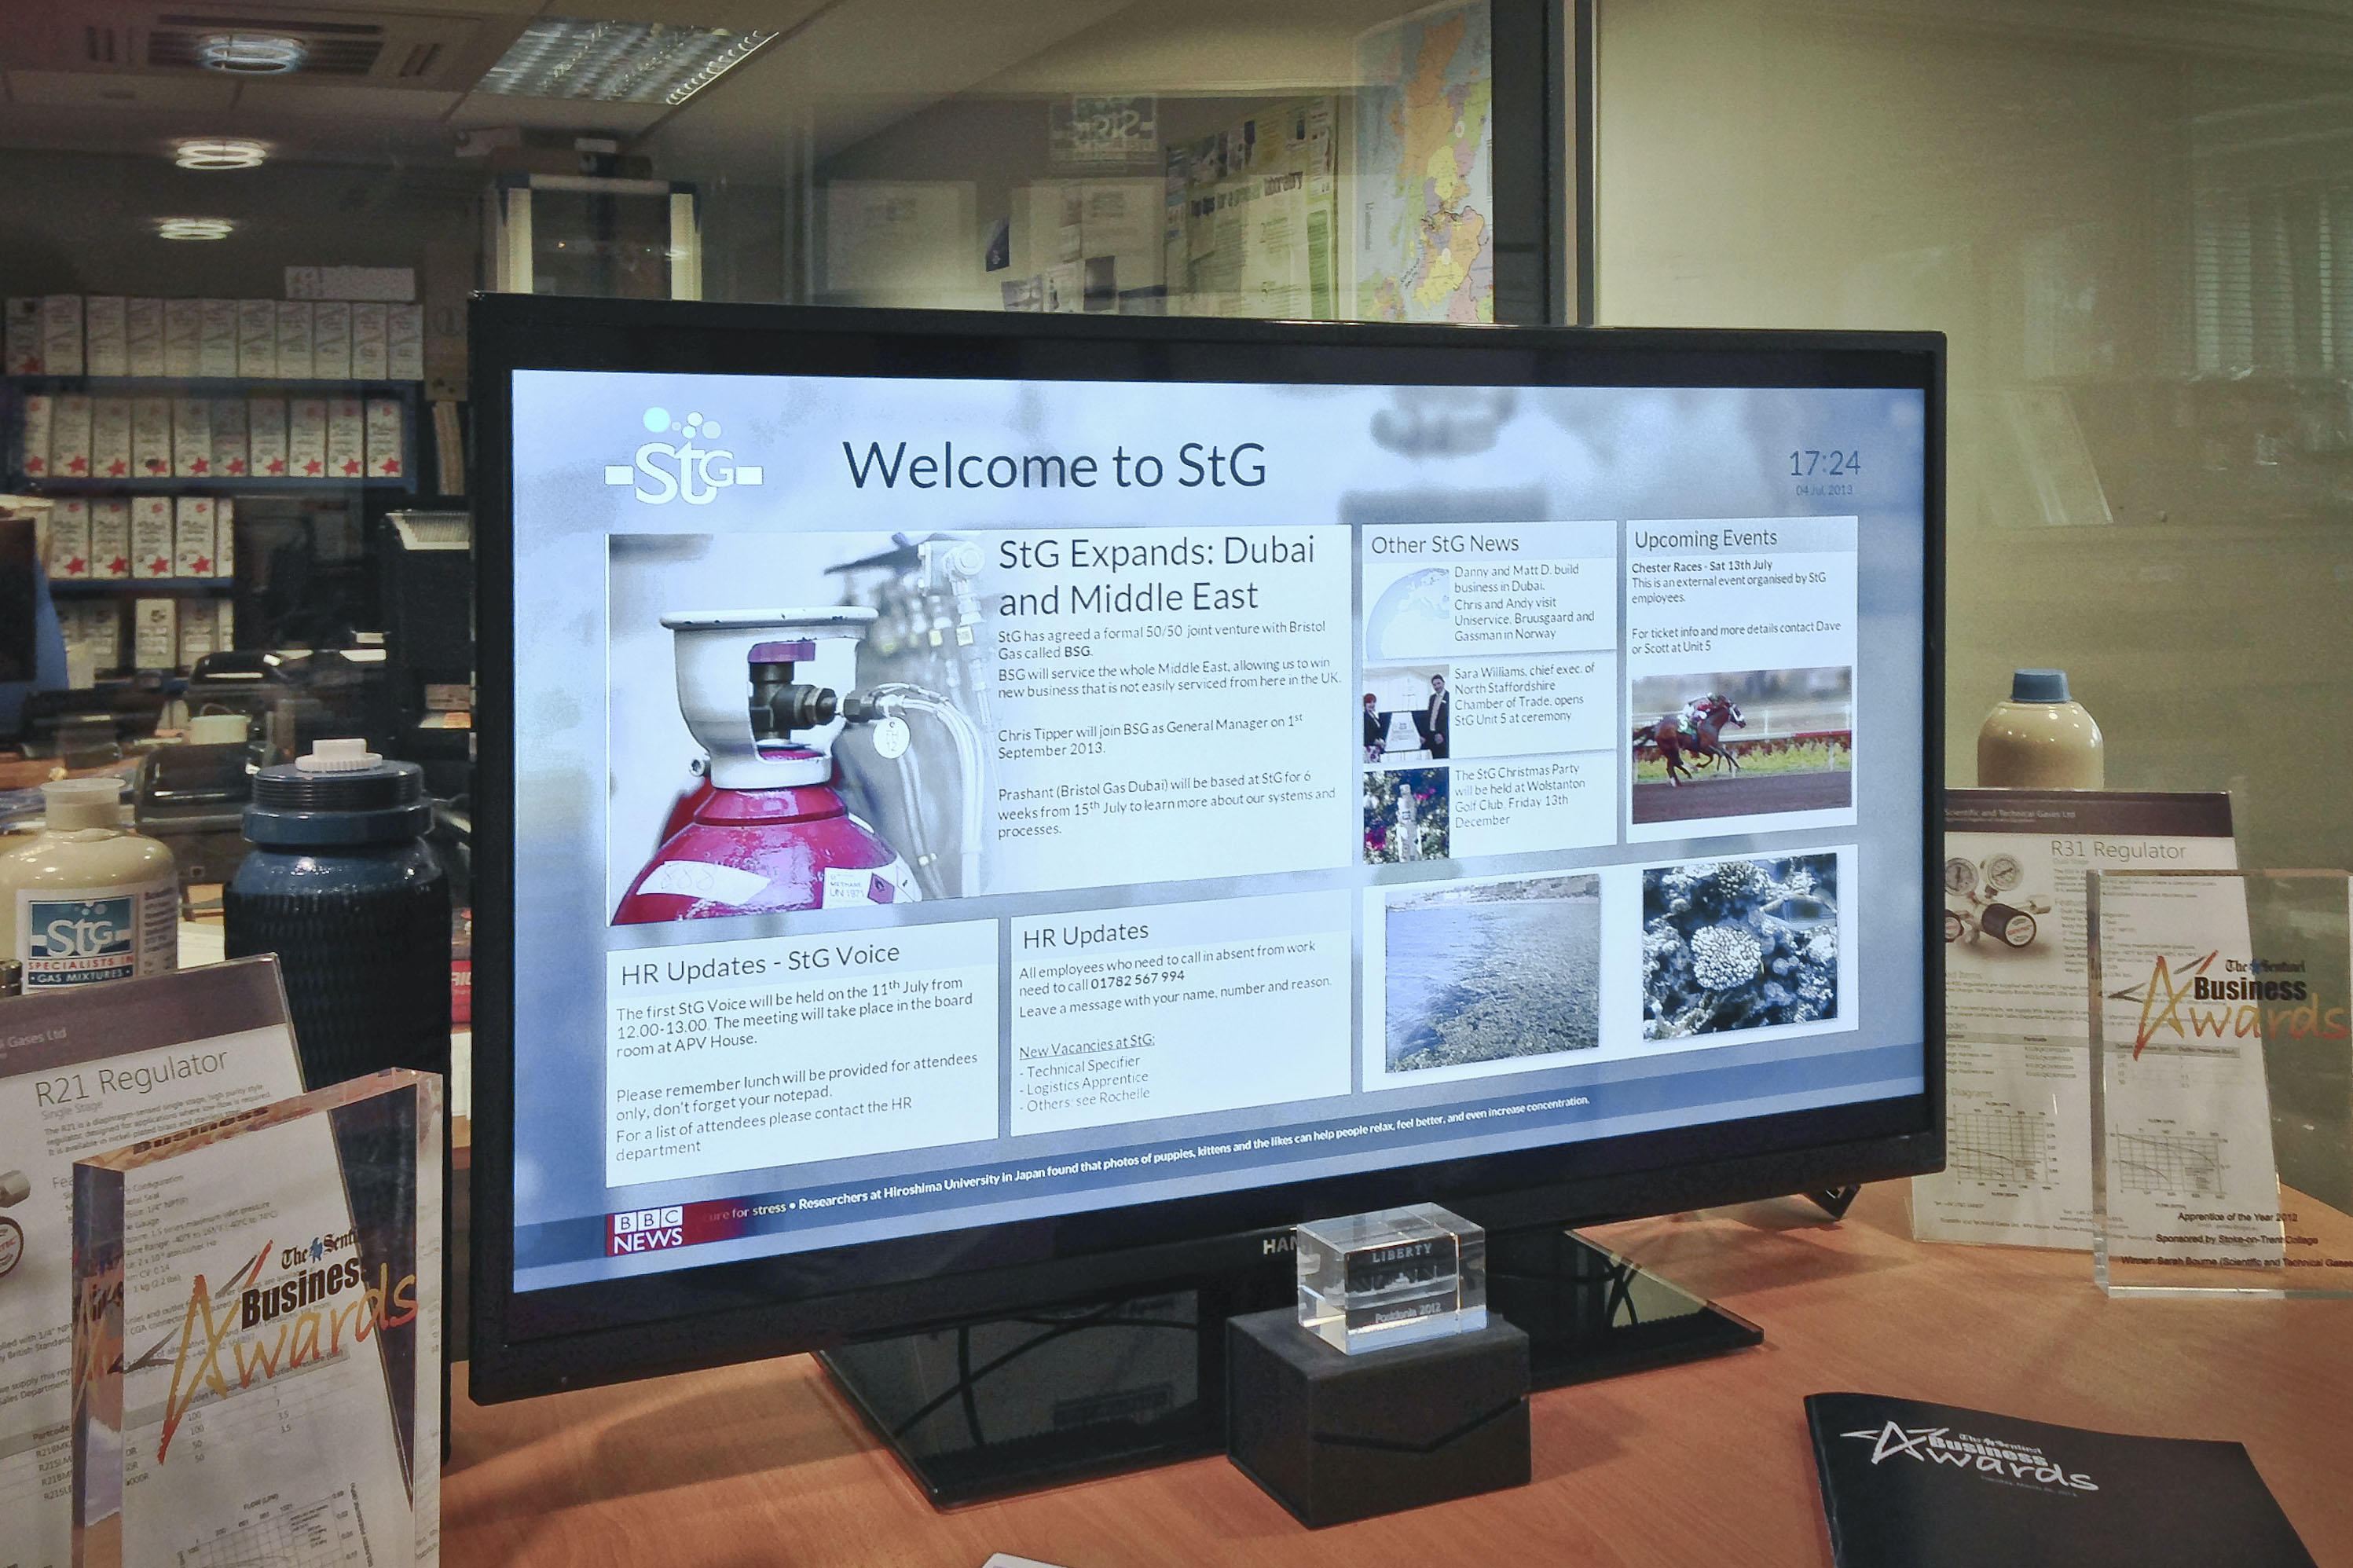
\includegraphics[width=9cm]{uc/board.jpg}

\medskip
\url{https://pipresents.wordpress.com/}
\end{center}
\end{frame}

\begin{frame}{Torrent Server}
\begin{center}
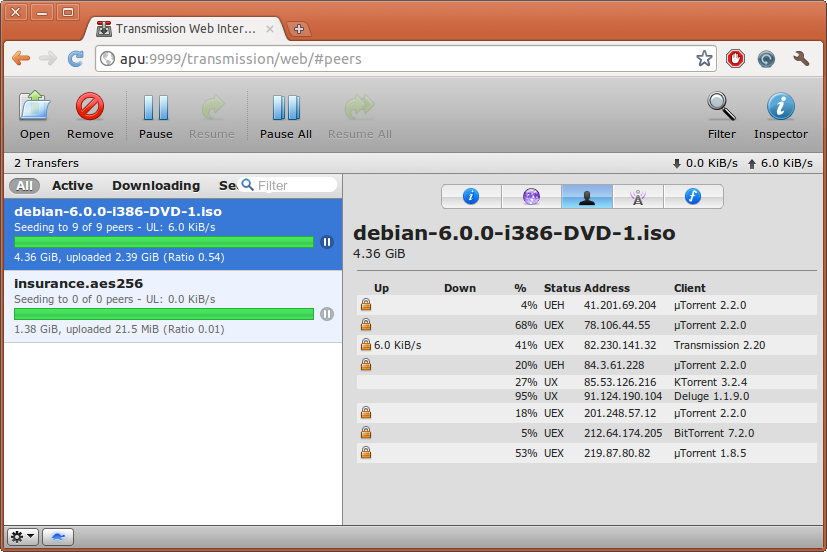
\includegraphics[width=9cm]{uc/torrent.png}
\end{center}
\end{frame}

\begin{frame}{NAS}
\begin{center}
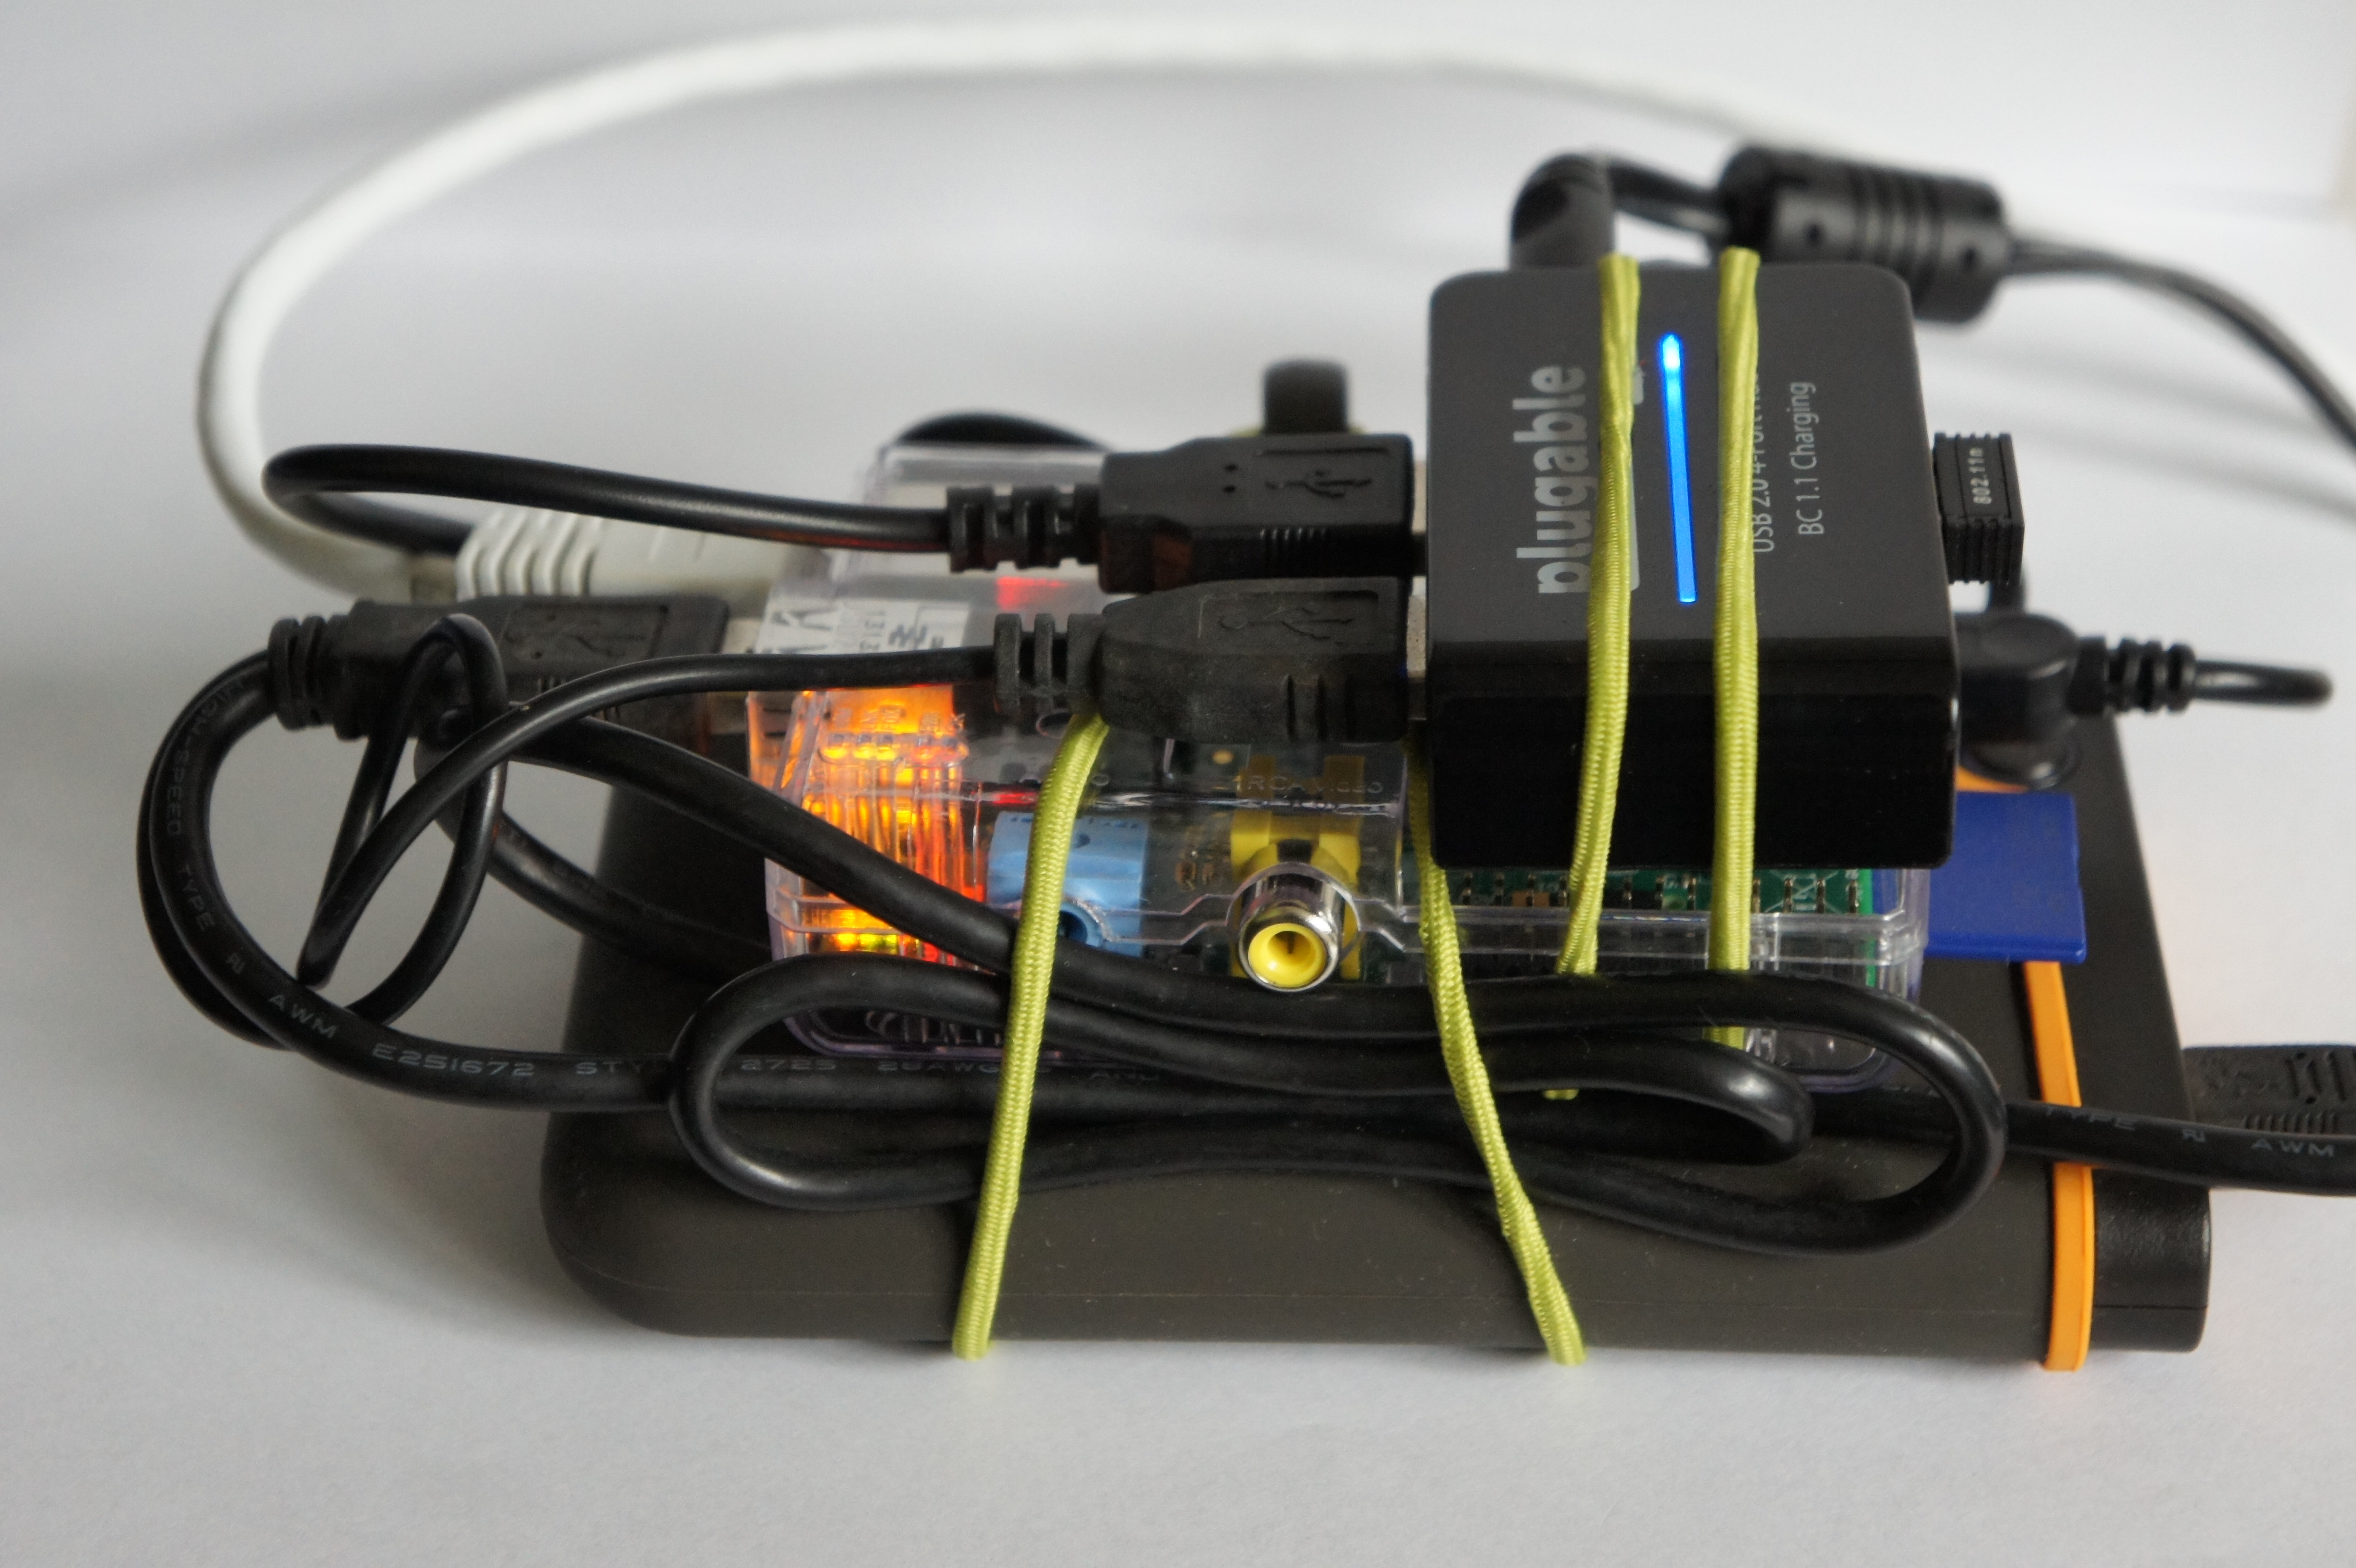
\includegraphics[width=9cm]{uc/nas.jpg}
\newline
\medskip
\url{https://owncloud.org/}
\end{center}
\end{frame}

\begin{frame}{Home security}
\begin{center}
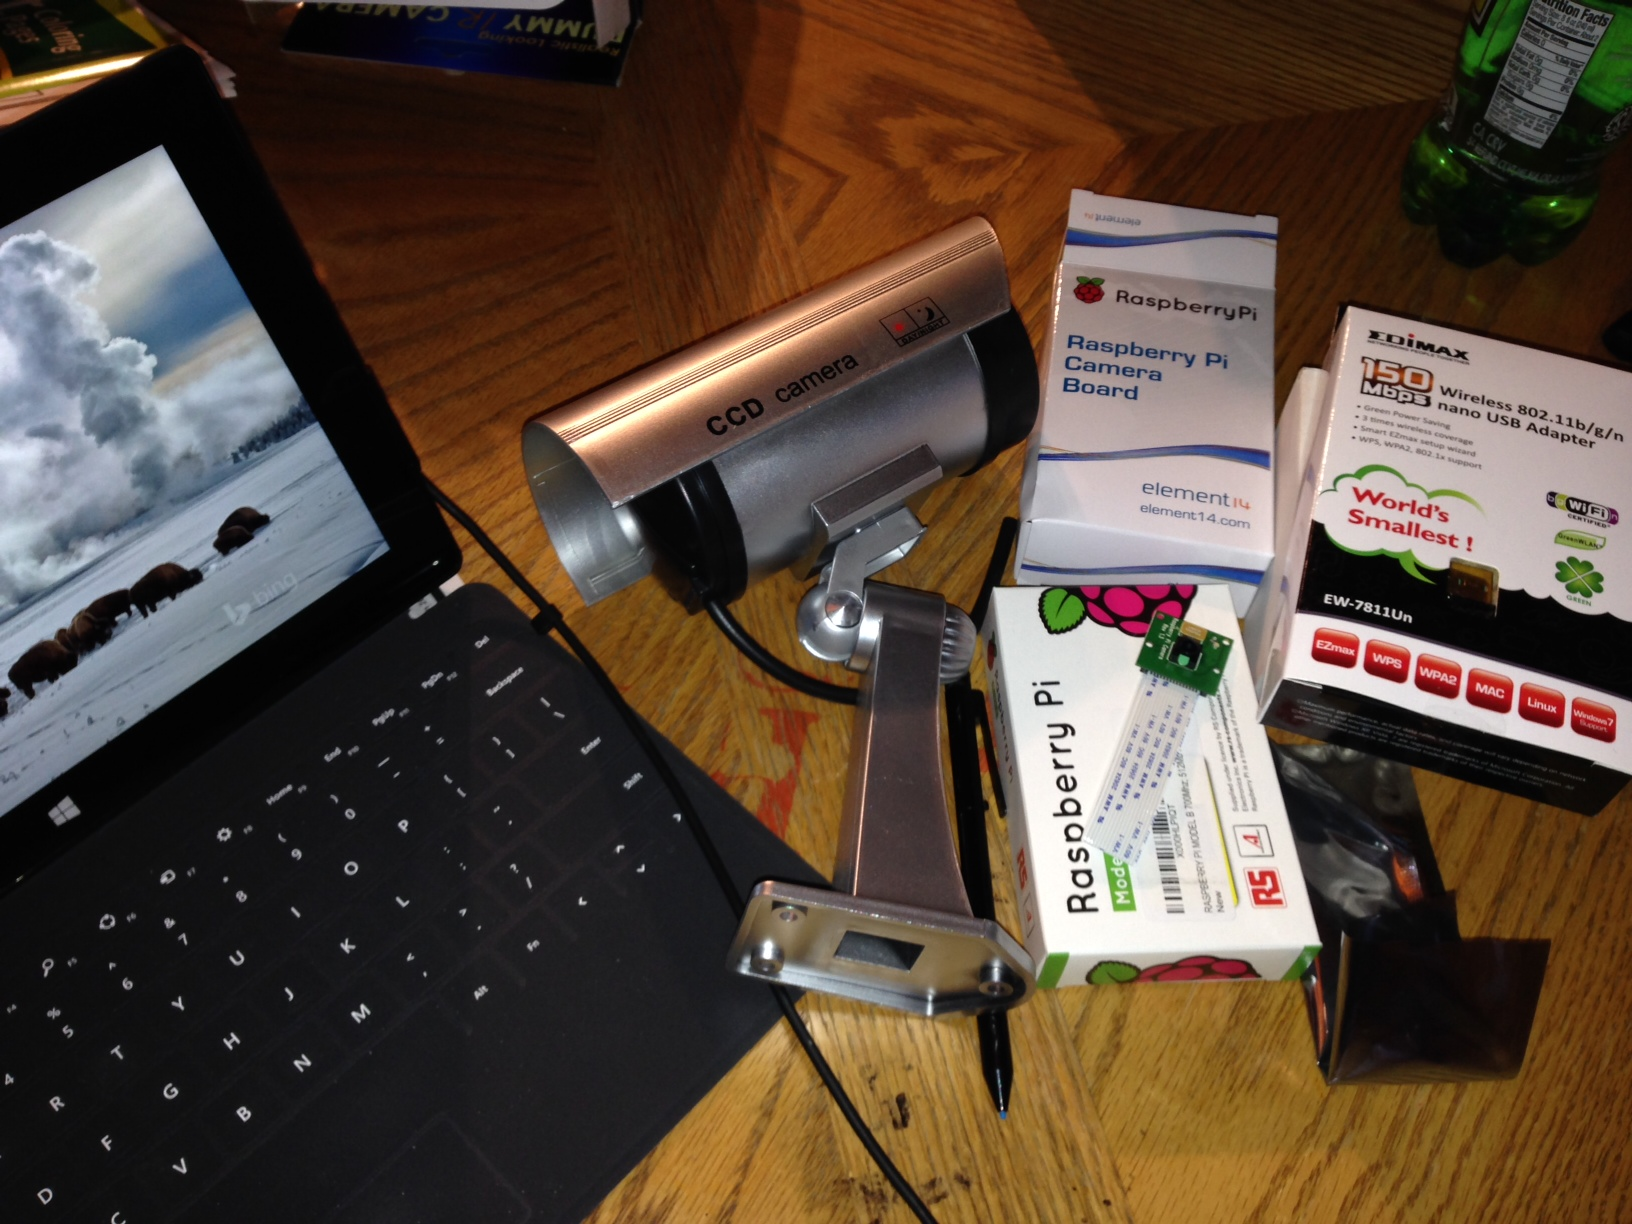
\includegraphics[width=9cm]{uc/security.jpg}
\newline
\medskip
\url{http://www.projects.privateeyepi.com/}
\end{center}
\end{frame}

\begin{frame}{Scratch}
\begin{center}
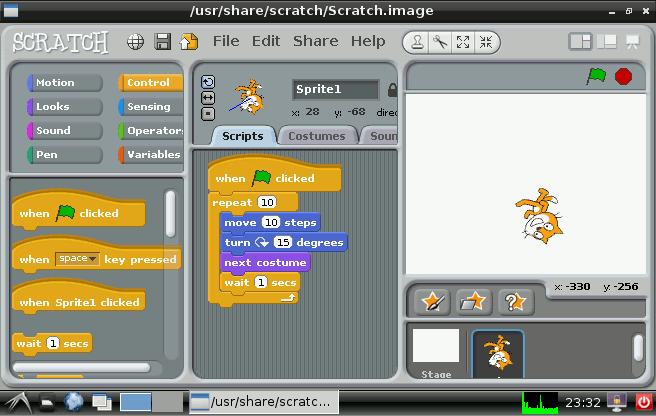
\includegraphics[width=9cm]{uc/scratch.png}
\newline
\medskip
\url{https://scratch.mit.edu/}
\end{center}
\end{frame}

\begin{frame}{Arcade box}
\begin{center}
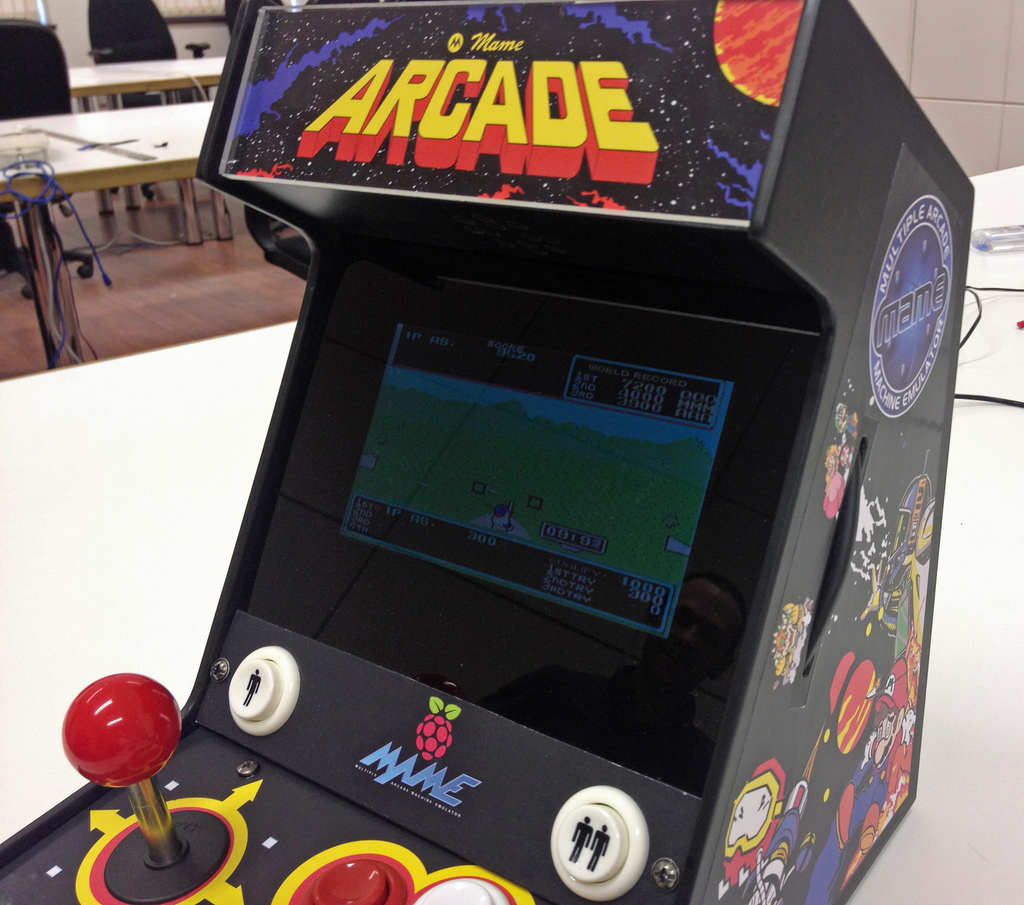
\includegraphics[width=9cm]{uc/arcade.jpg}
\end{center}
\end{frame}

\begin{frame}{Arcade box}
\begin{center}
\url{http://pimame.org/}
\end{center}
\begin{itemize}
\begin{footnotesize}
\item MAME - AdvanceMAME \& MAME4ALL
\item CPS I / CPS II - Final Burn Alpha
\item Neo Geo - GNGeo
\item Playstation - pcsx-reARMed
\item Genesis - DGen
\item SNES - SNES9x
\item NES - AdvMESS
\item Gameboy - Gearboy
\item Gameboy Advance - GPSP
\item ScummVM
\item Atari 2600 - Stella
\item Cavestory - NXEngine
\item Commodore 64 - VICE

\end{footnotesize}
\end{itemize}
\end{frame}


\begin{frame}{Altro...}
\begin{center}
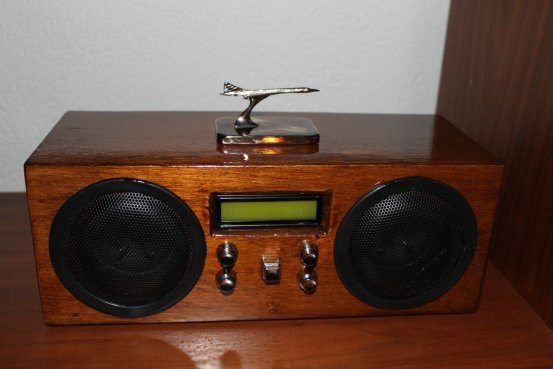
\includegraphics[width=9cm]{uc/radio.jpg}
\medskip
\newline
\url{http://www.woutervanwijk.nl/pimusicbox/}
\end{center}
\end{frame}

\begin{frame}{Altro...}
\begin{center}
\includegraphics<1>[width=9cm]{uc/cluster.jpg}
\includegraphics<2>[width=9cm]{uc/keyboard.jpg}
\includegraphics<3>[width=9cm]{uc/drone.jpg}

\end{center}
\end{frame}

\section{Prima installazione}

\begin{frame}{}
\begin{center}
\begin{Huge}
{\color{green_raspi} \textbf{Prima installazione}}
\end{Huge}
\end{center}
\end{frame}

\begin{frame}{Prima installazione}
\begin{block}{NOOBS}

Per la prima installazione consiglio di usare \textbf{NOOBS} (New Out Of the Box Software), un manager che ci aiuta durante l'installazione del nostro sistema operativo.

\end{block}

\pause
\medskip

NOOBS \`e sviluppato direttamente dalla Raspberry Pi Foundation, e sono presenti numerose guide che ci guideranno passo passo nella configurazione.

\pause
\medskip
\begin{center}
\url{http://www.raspberrypi.org/help/noobs-setup/}
\end{center}

\pause
\medskip

Si possono anche acquistare schede SD con NOOBS \textbf{precaricato} all'interno.

\end{frame}

\begin{frame}{1) Scaricare NOOBS}
Scaricare NOOBS dal sito internet
\begin{center}
\url{http://www.raspberrypi.org/downloads/}

\bigskip
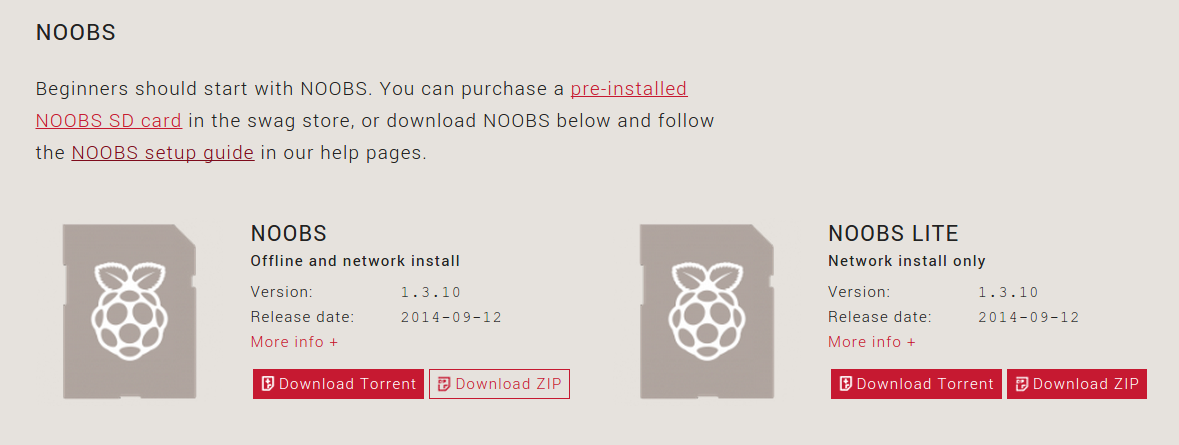
\includegraphics[width=8cm]{guide/1.png}

\end{center}
\end{frame}

\begin{frame}{2) Formattare la scheda SD}
Formattare una scheda SD da almeno \textbf{4 GB} e creare una nuova partizione con filesystem \textbf{FAT32}.

\bigskip
\begin{center}
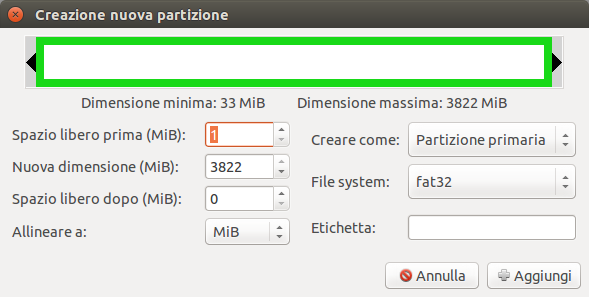
\includegraphics[width=8cm]{guide/2.png}
\end{center}
\end{frame}

\begin{frame}{3) Copiare NOOBS su scheda SD}
Copiare il contenuto dell'archivio di NOOBS dentro la scheda SD (nella root, cio\`e senza creare cartelle).

\medskip
\begin{center}
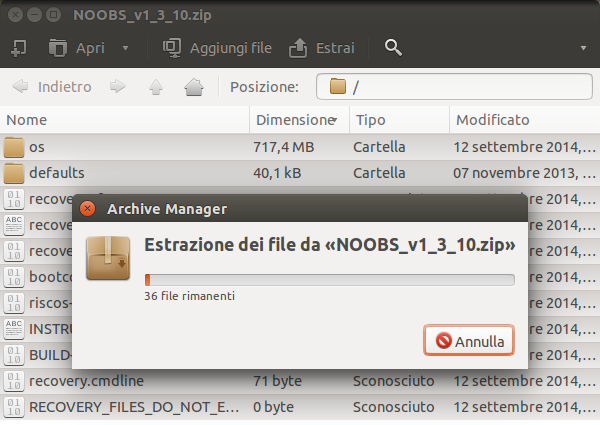
\includegraphics[width=8cm]{guide/3.png}
\end{center}
\end{frame}

\begin{frame}{4) Avviare il Raspberry Pi}
Inserire la scheda SD nel Raspberry Pi, collegare le periferiche (monitor, tastiera, etc...), collegare la rete, ed attaccare il raspberry all'alimentazione.

\medskip
\begin{center}
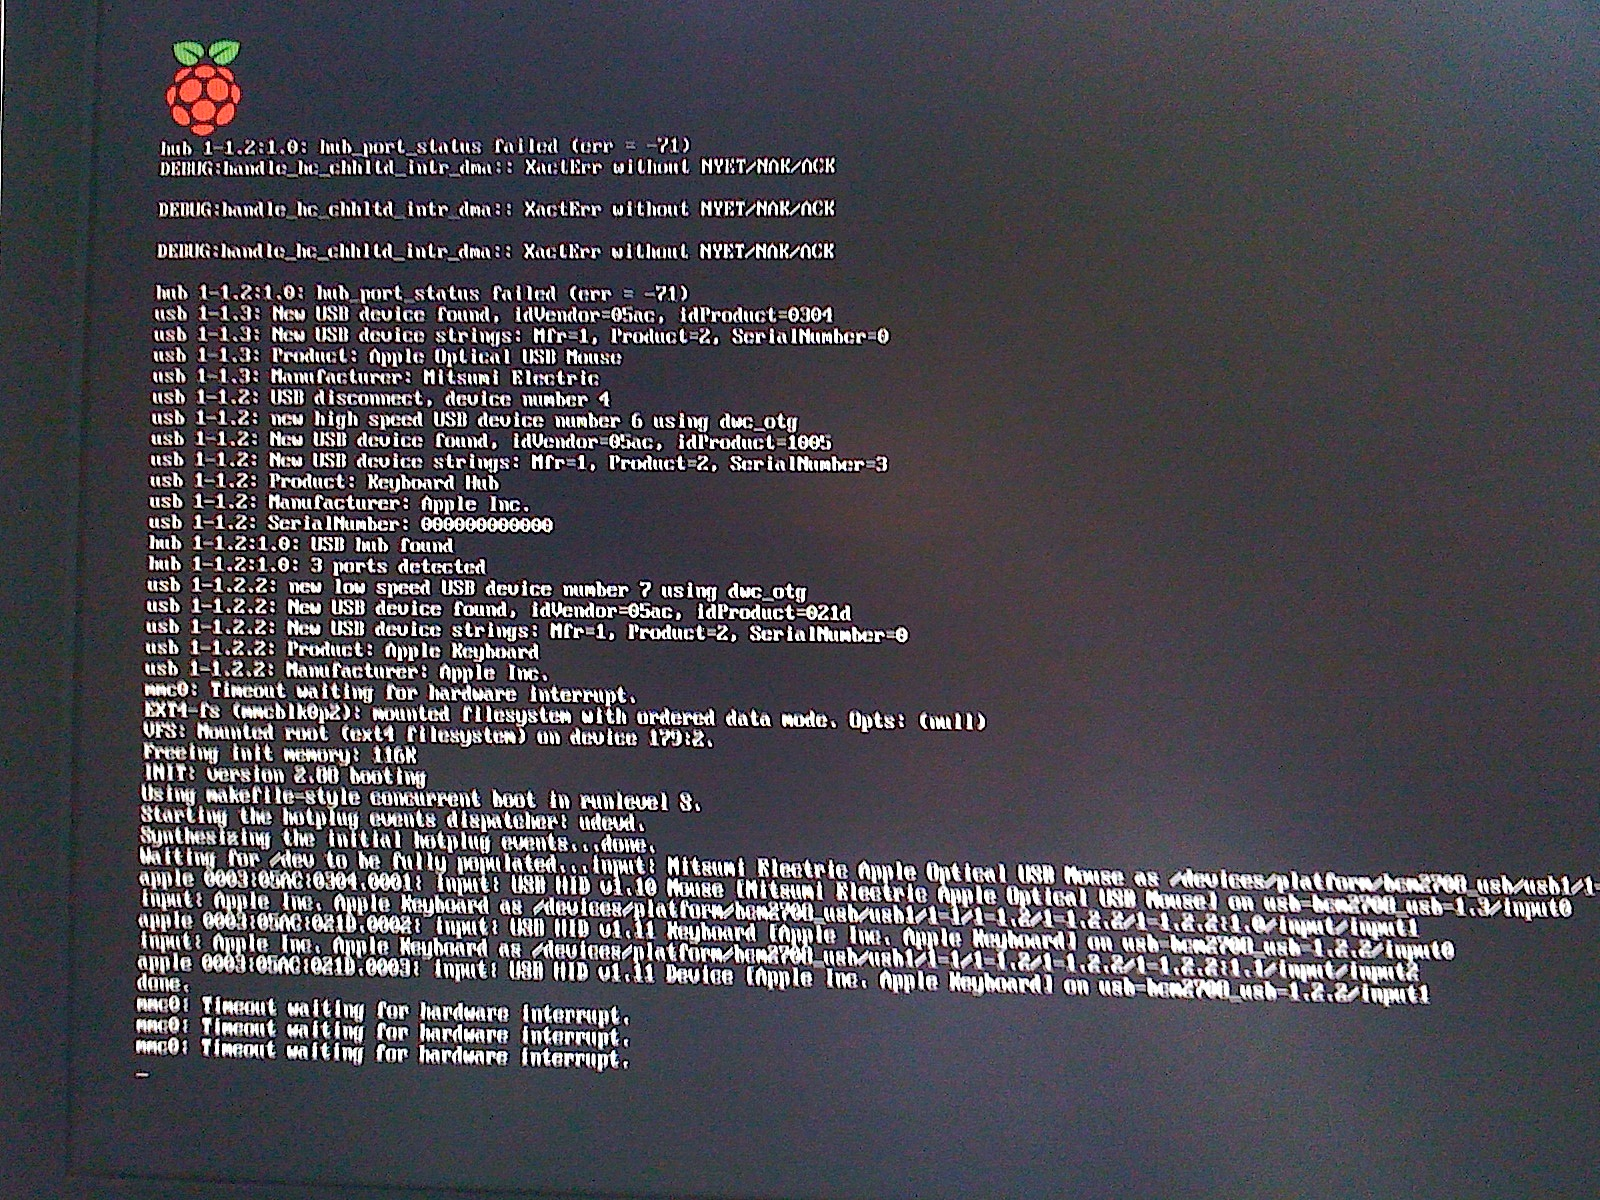
\includegraphics[width=8cm]{guide/4.jpg}
\end{center}
\end{frame}



\begin{frame}{5) Scegliere i S.O.}
Scegliere dall'elenco di Sistemi Operativi che si vogliono installare su questa scheda SD.

\medskip
\begin{center}
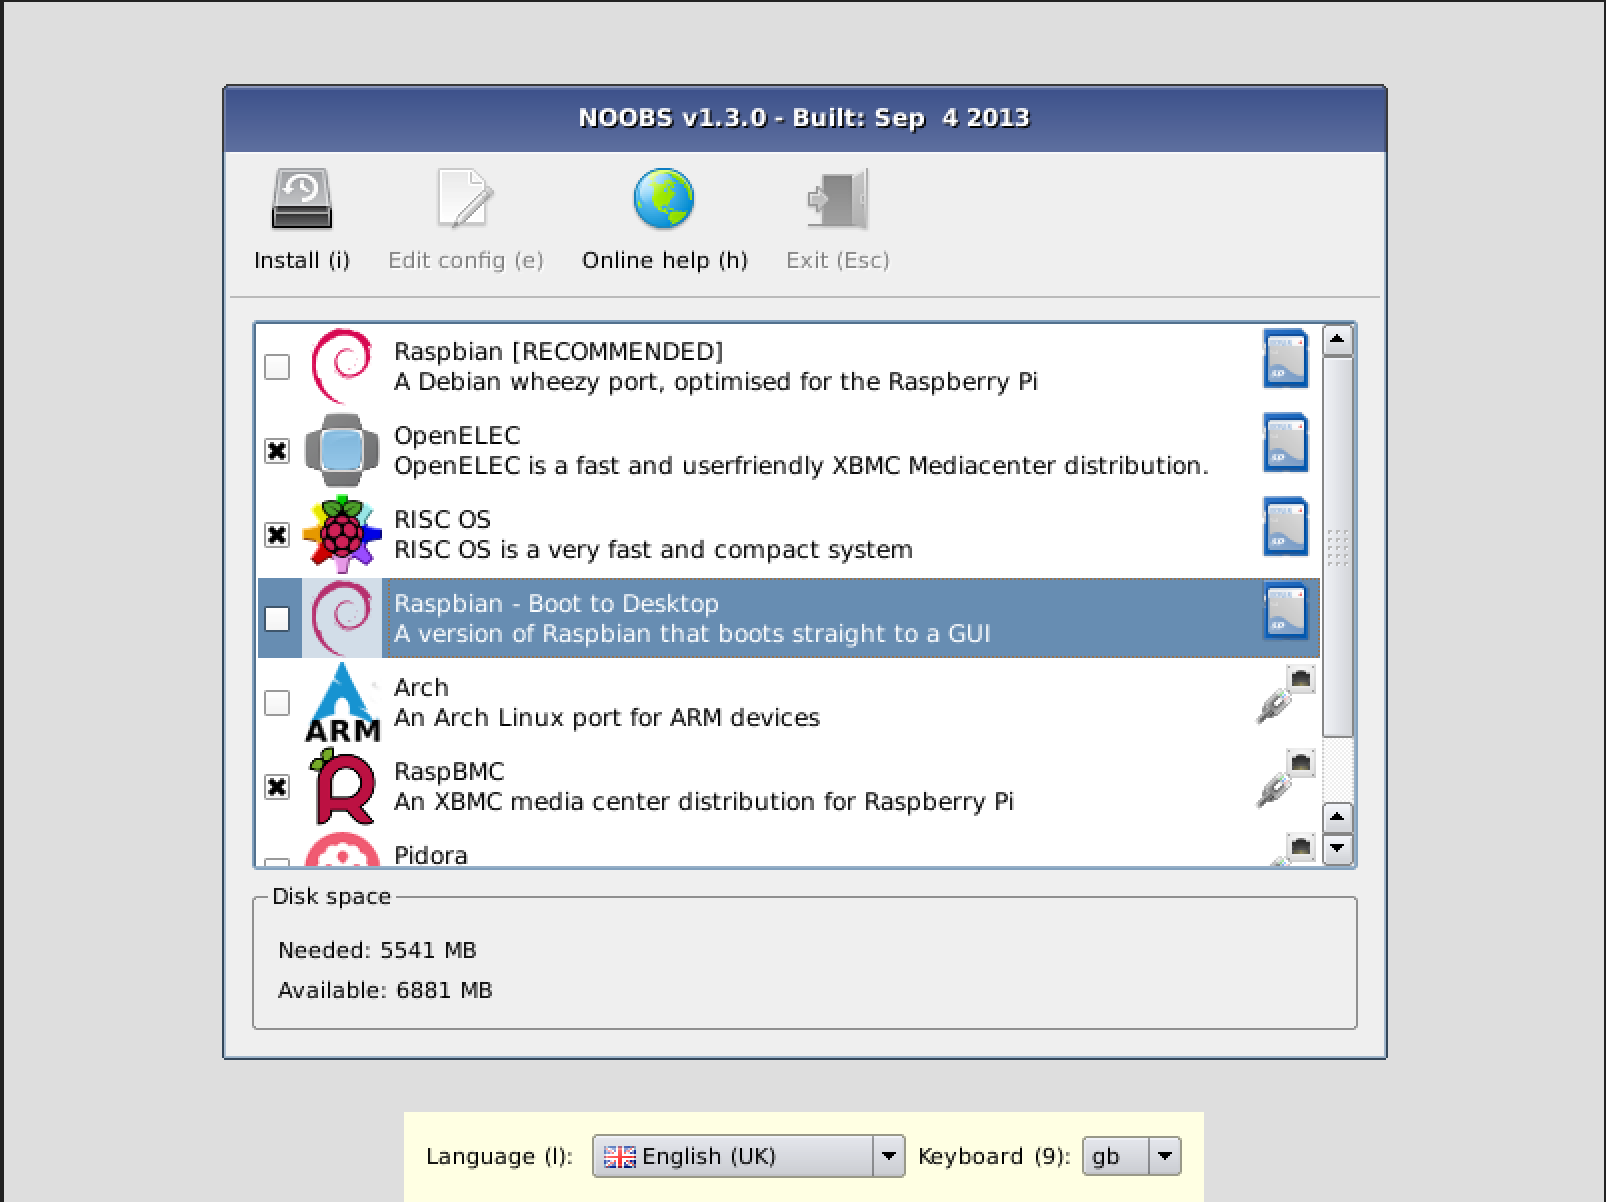
\includegraphics[width=8cm]{guide/5.png}
\end{center}

All'avvio potremo scegliere quale sistema avviare

\end{frame}


\begin{frame}{6) Attendere...}
Attendi che il Raspberry Pi scarichi da internet tutti i sistemi operativi che hai scelto.

\medskip
\begin{center}
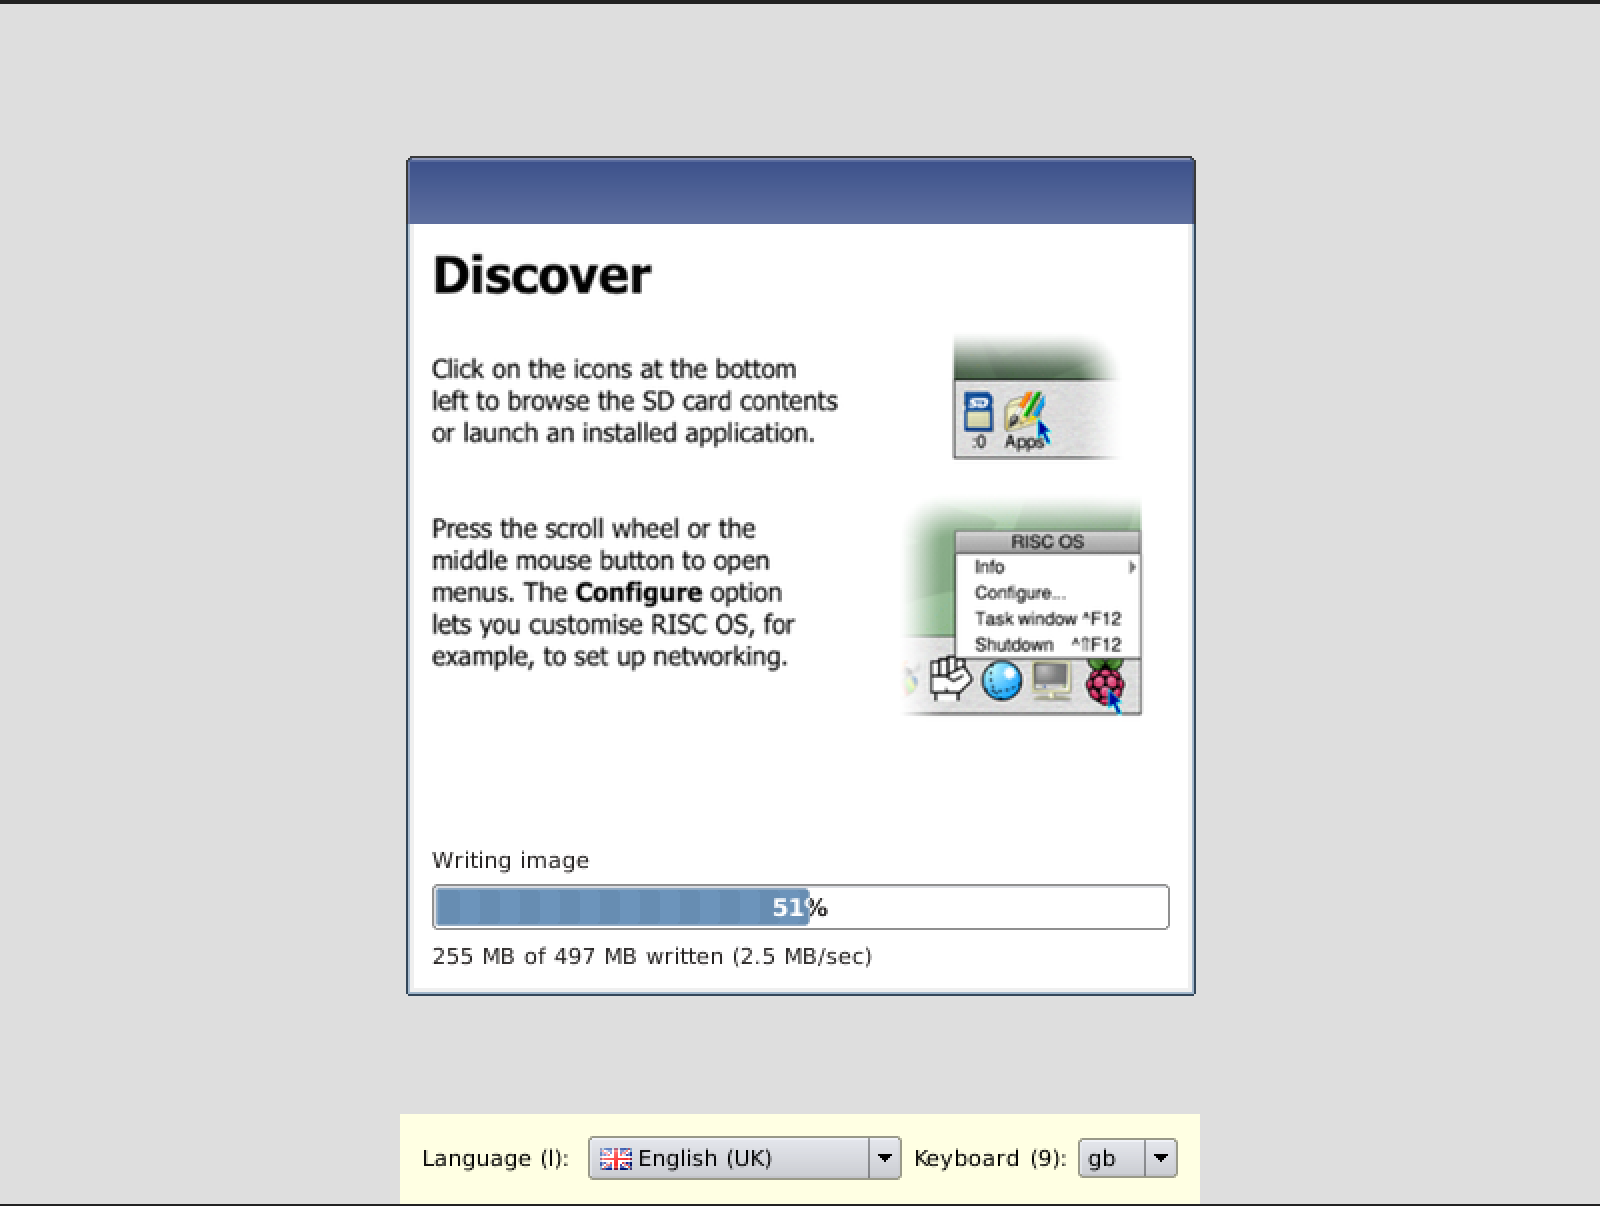
\includegraphics[width=8cm]{guide/6.png}
\end{center}
\end{frame}

\section{Riferimenti}
\begin{frame}{Cookbook}
\begin{center}
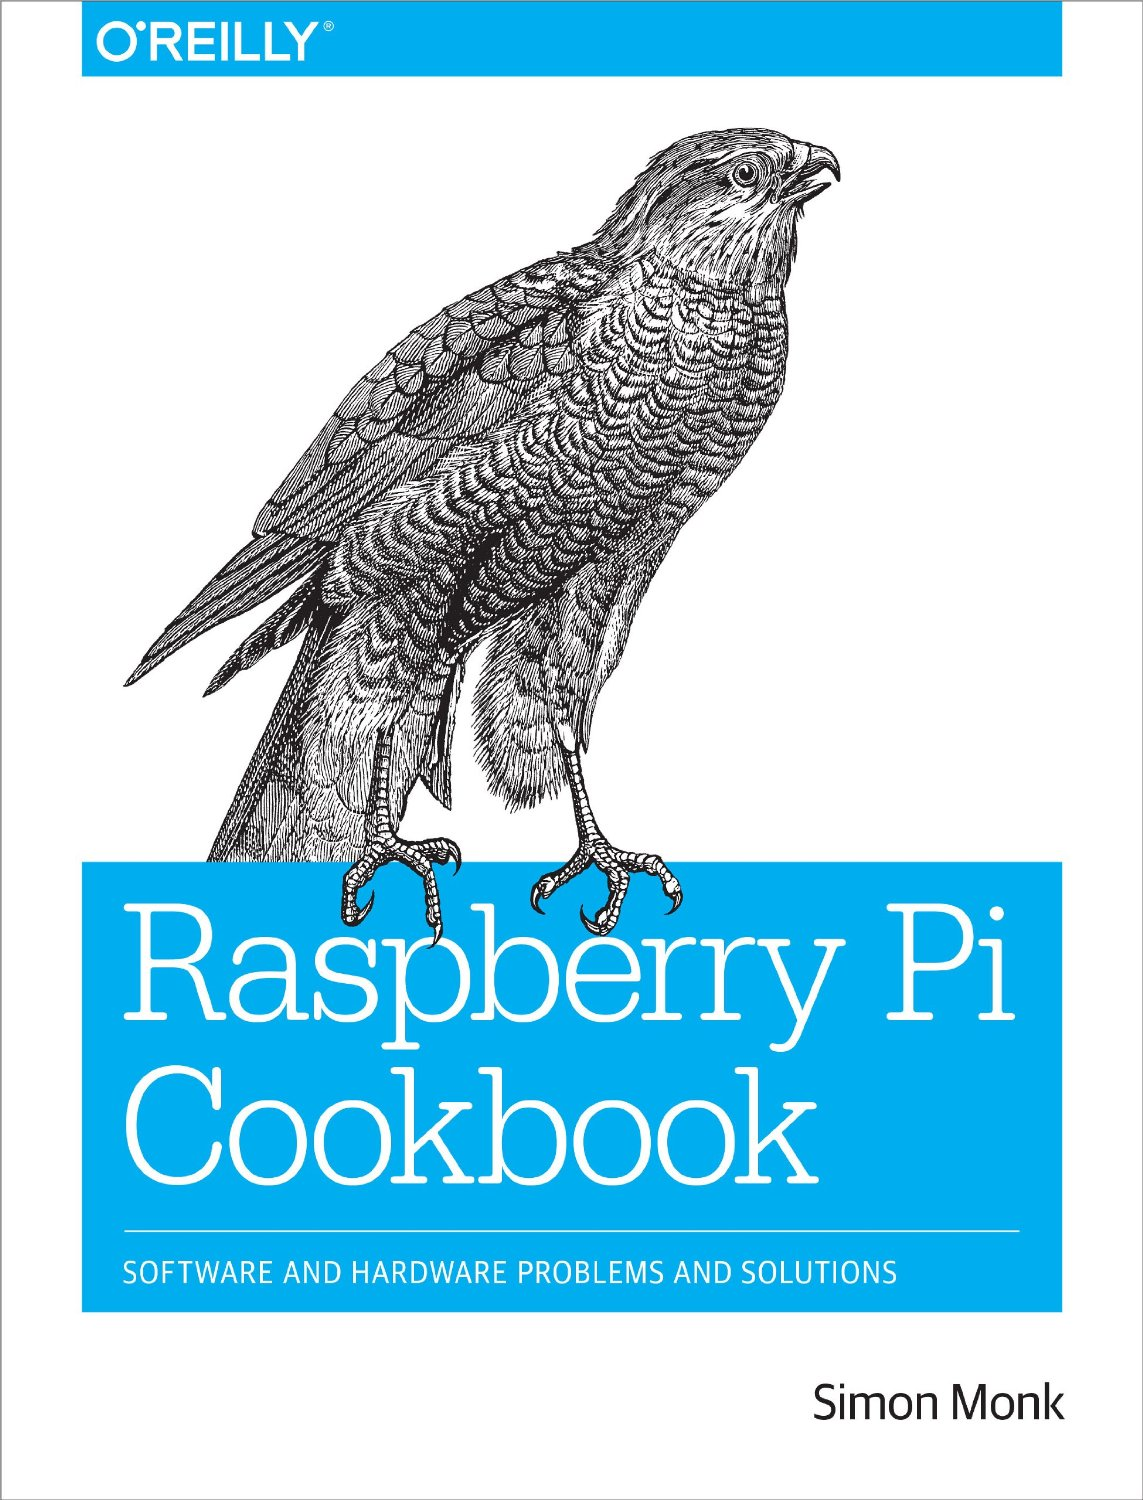
\includegraphics[width=5cm]{book.jpg}
\medskip
\newline
\url{http://it-ebooks.info/book/3175/}
\end{center}
\end{frame}

\begin{frame}{Web}
\begin{enumerate}
\begin{footnotesize}
\item \url{https://www.raspberrypi.org/}
\item \url{https://www.raspberrypi.org/help/quick-start-guide/}
\item \url{https://www.raspberrypi.org/help/noobs-setup/}
\item \url{http://elinux.org/RPi_Hub}
\item \url{http://www.raspbian.org/RaspbianDocumentation}
\end{footnotesize}
\end{enumerate}
\end{frame}

\begin{frame}{}
\begin{center}
\begin{Huge}
{\color{green_raspi} \textbf{Domande...?}}
\end{Huge}

\vspace{1.5cm}
\begin{small}
Slides realizzate da:\\
\textbf{Nicola Corti - corti.nico [at] gmail [dot] com}\\

\bigskip

Slides realizzate con \LaTeX\ Beamer.\\
La seguente presentazione \`e rilasciata sotto licenza\\
\begin{footnotesize}	\textbf{Creative Commons - Attributions, Non Commercial, Share-alike}.
\end{footnotesize}
\\
\medskip

\includegraphics[height=0.5cm]{cc.png}

\end{small}
\end{center}
\end{frame}

\end{document}
